%
% main.tex
%
% Copyright (C) 2021 by SpaceLab.
%
% EPS 2.0 Documentation
%
% This work is licensed under the Creative Commons Attribution-ShareAlike 4.0
% International License. To view a copy of this license,
% visit http://creativecommons.org/licenses/by-sa/4.0/.
%

%
% \brief Main file.
%
% \author Gabriel Mariano Marcelino <gabriel.mm8@gmail.com>
%
% \institution Universidade Federal de Santa Catarina (UFSC)
%
% \version 0.2.0
%
% \date 2020/11/05
%

\documentclass[a4paper,12pt]{book}

\usepackage{spacelab_book}

\title{EPS 2.0 Documentation}
\author{SpaceLab}
\date{\today}

% File metadata
\hypersetup
{
    pdfauthor   = {SpaceLab},
    pdfsubject  = {\thetitle},
    pdftitle    = {\thetitle},
    pdfkeywords = {Nanosatellites, CubeSats, Electric Power System}
}

\begin{document}

    \pagenumbering{roman}
    \setcounter{page}{1}

    %
% titlepage.tex
%
% Copyright (C) 2020 by SpaceLab.
%
% EPS 2.0 Documentation
%
% This work is licensed under the Creative Commons Attribution-ShareAlike 4.0
% International License. To view a copy of this license,
% visit http://creativecommons.org/licenses/by-sa/4.0/.
%

%
% \brief Title page.
%
% \author Gabriel Mariano Marcelino <gabriel.mm8@gmail.com>
%
% \institution Universidade Federal de Santa Catarina (UFSC)
%
% \version 0.1.0
%
% \date 2020/11/05
%

\begin{titlepage}

\thispagestyle{empty}

\begin{flushleft}
SLB-EPS2-DOC-v0.1
\end{flushleft}

\begin{figure}[!ht]
    \begin{flushleft}
        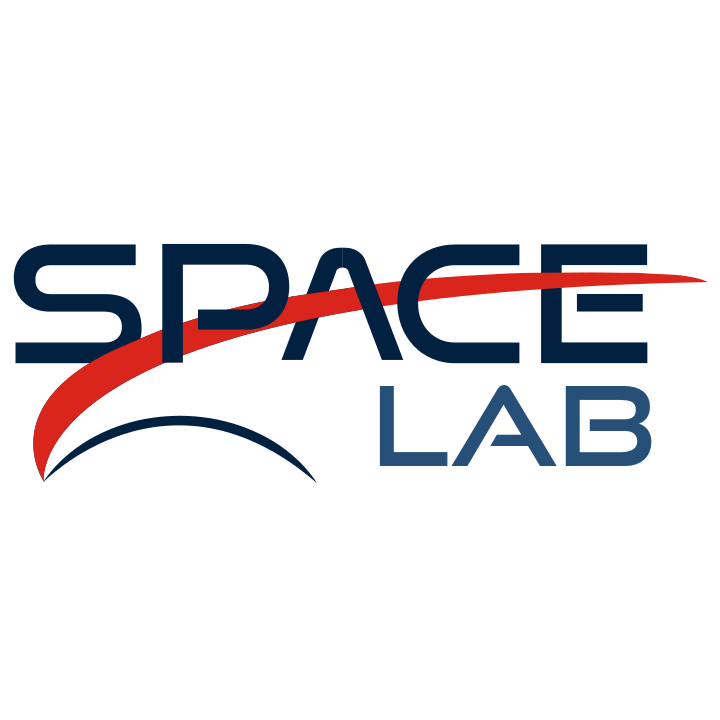
\includegraphics[width=5cm]{figures/spacelab.png}
    \end{flushleft}
\end{figure}

\begin{flushleft}
\Huge{\textbf{\thetitle}}
\rule[0pt]{\textwidth}{5pt}
\end{flushleft}

\vspace{0.2cm}

\begin{flushleft}
\textit{\thetitle} \\
\textit{SpaceLab, Universidade Federal de Santa Catarina, Florianópolis - Brazil}
\end{flushleft}

\vfill
\vfill

\begin{flushright}
November 2020
\end{flushright}

\end{titlepage}

    \cleardoublepage
    %
% authorpage.tex
%
% Copyright (C) 2021 SpaceLab.
%
% EPS 2.0 Documentation
%
% This work is licensed under the Creative Commons Attribution-ShareAlike 4.0
% International License. To view a copy of this license,
% visit http://creativecommons.org/licenses/by-sa/4.0/.
%

%
% \brief Author page.
%
% \author Gabriel Mariano Marcelino <gabriel.mm8@gmail.com>
% \author Yan Castro de Azeredo <yan.ufsceel@gmail.com>
%
% \institution Universidade Federal de Santa Catarina (UFSC)
%
% \version 0.2
%
% \date 2021/06/07
%

\thispagestyle{empty}

\begin{center}

\textbf{\thetitle}

\textit{June, 2021}

\vspace{1cm}

\textbf{Project Chief:}

Eduardo Augusto Bezerra <\href{mailto:eduardo.bezerra@spacelab.ufsc.br}{eduardo.bezerra@spacelab.ufsc.br}>

\vspace{1cm}

\textbf{Authors:}

André Martins Pio de Mattos <\href{mailto:andre.mattos@spacelab.ufsc.br}{andre.mattos@spacelab.ufsc.br}>\\
Gabriel Mariano Marcelino <\href{mailto:gabriel.marcelino@spacelab.ufsc.br}{gabriel.marcelino@spacelab.ufsc.br}>\\
Yan Castro de Azeredo <\href{mailto:yan.azeredo@spacelab.ufsc.br}{yan.azeredo@spacelab.ufsc.br}>\\
Augusto Cezar Boldori Vassoler \\ 
Vinicius Pimenta Bernardo \\

\vspace{1cm}

\textbf{Contributing Authors:}

Leonardo Kessler Slongo \\
Sara Vega Martinez \\
Bruno Vale Barbosa Eiterer \\
Túlio Gomes Pereira \\

\vspace{1cm}


\textbf{Revision Control:}

\end{center}

\begin{table}[!ht]
    \begin{center}
        \begin{tabular}{cL{5cm}L{5.5cm}C{2cm}}
            \toprule[1.5pt]
            \textbf{Version} & \textbf{Author}  & \textbf{Changes}    & \textbf{Date} \\
            \midrule
            0.1     & G. Marcelino              & Document creation   & 2020/11/05 \\
            0.2     & Y. C. Azeredo, G. Marcelino & First stable hardware & TBD   \\
                    &                           &                     &            \\
                    &                           &                     &            \\
            \bottomrule[1.5pt]
        \end{tabular}
    \end{center}
\end{table}

\vfill

\begin{figure}[!h]
	\begin{center}
		
\includegraphics[width=0.25\textwidth]{figures/by-sa.pdf}
	\end{center}
\end{figure}

\textcopyright\  2021 by SpaceLab. \thetitle. This work is licensed under the Creative Commons Attribution-ShareAlike 4.0 International License. To view a copy of this license, visit \href{http://creativecommons.org/licenses/by-sa/4.0/}{http://creativecommons.org/licenses/by-sa/4.0/}.

    \cleardoublepage

    \listoffigures
    \addcontentsline{toc}{chapter}{List of Figures}

    \listoftables
    \addcontentsline{toc}{chapter}{List of Tables}

    \printnomenclature
    \addcontentsline{toc}{chapter}{Nomenclature}

    \tableofcontents
    \cleardoublepage
    
    \pagenumbering{arabic}
    \setcounter{page}{1}

    %
% introduction.tex
%
% Copyright (C) 2021 by SpaceLab.
%
% EPS 2.0 Documentation
%
% This work is licensed under the Creative Commons Attribution-ShareAlike 4.0
% International License. To view a copy of this license,
% visit http://creativecommons.org/licenses/by-sa/4.0/.
%

%
% \brief Introduction chapter.
%
% \author Gabriel Mariano Marcelino <gabriel.mm8@gmail.com>
% \author Yan Castro de Azeredo <yan.ufsceel@gmail.com>
%
% \institution Universidade Federal de Santa Catarina (UFSC)
%
% \version 0.2.0
%
% \date 2021/03/16
%

\chapter{Introduction} \label{ch:introduction}

The EPS 2.0\nomenclature{\textbf{EPS}}{\textit{Electric Power System.}} is a PCB\nomenclature{\textbf{PCB}}{\textit{Printed Circuit Board.}} designed to harvest, store and distribute energy for a nanosatellite. It is one of the service modules developed for FloripaSat-2 CubeSat Mission \cite{floripasat2-doc}. The energy harvesting system is based on solar energy conversion through ten solar panels attached to the 2U CubeSat structure. The EPS 2.0 is designed to operate the solar panels at their maximum power point (MPPT)\nomenclature{\textbf{MPPT}}{\textit{Maximum Power Point Tracking.}}. The board is also responsible for measuring solar panels current, voltage and the temperature of the panels and batteries. The harvested solar energy is stored in the Battery Module 4C \cite{bat4c} connected to the EPS. The energy distribution is done by several integrated buck DC-DC converters. The full EPS system is composed of the solar panels, the EPS 2.0 PCB and the battery module. A general view of the EPS 2.0 board can be seen in \autoref{fig:general-view}.

The module is a direct upgrade from the EPS of FloripaSat-1 \cite{eps-fsat}, which grants a flight heritage rating. The improvements focus on providing a cleaner and more generic implementation in comparison with the previous version, more reliability in software, and adaptations for the new mission requirements. All the project, source and documentation files are available freely on a GitHub repository \cite{eps2} under its respective licenses.

\begin{figure}[!ht]
    \begin{center}
        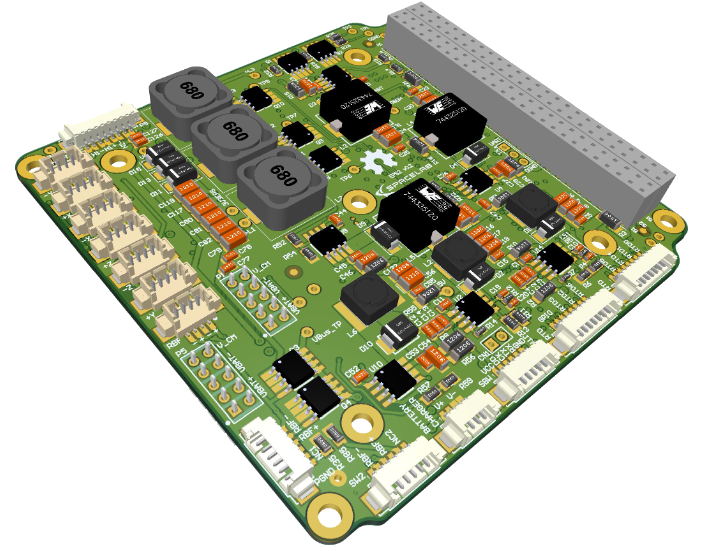
\includegraphics[width=0.55\textwidth]{figures/eps2-pcb-3d}
        \caption{3D view of the EPS 2.0 PCB.}
        \label{fig:general-view}
    \end{center}
\end{figure}
    %
% system_overview.tex
%
% Copyright The EPS 2.0 Contributors.
%
% EPS 2.0 Documentation
%
% This work is licensed under the Creative Commons Attribution-ShareAlike 4.0
% International License. To view a copy of this license,
% visit http://creativecommons.org/licenses/by-sa/4.0/.
%

%
% \brief System overview chapter.
%
% \author Gabriel Mariano Marcelino <gabriel.mm8@gmail.com>
% \author Yan Castro de Azeredo <yan.ufsceel@gmail.com>
%
% \version 0.3.0
%
% \date 2021/02/10
%

\chapter{System Overview} \label{ch:system-overview}

The board has a MSP430 low-power MCU\nomenclature{\textbf{MCU}}{\textit{Microcontroller.}} that runs the firmware application intended to control and communicate with its peripherals, subsystems, and other modules. The programming language used is C, and the firmware was developed using the Code Composer Studio IDE\nomenclature{\textbf{IDE}}{\textit{Integrated Development Environment.}} (a.k.a. CCS) for compiling, programming and testing. The module has many tasks, such as interfacing internal peripherals and communicating with other boards over distinct protocols and time requirements. 
So, in order to improve predictability, a Real-Time Operating System (RTOS\nomenclature{\textbf{RTOS}}{\textit{Real Time Operating System.}}) is used to ensure that the deadlines are observed, even under a fault situation in a routine. The RTOS chosen is the FreeRTOS (v10.2.1) since it is designed for embedded systems applications and was already validated in space applications. The firmware architecture follows an abstraction layer scheme to facilitate higher level implementations and allow more portability across different hardware platforms; see \autoref{sec:system-layers} for more details.

The EPS 2.0 is compatible with GOMspace Solar Panels or with panels of similar characteristics. Algorithms are implemented to improve power generation through MPPT. Also, the load output can be regulated through measurements to achieve a more efficient power distribution to the nanosatellite.

\section{Product tree}

The product tree of the EPS 2.0 module is available in \autoref{fig:product-tree}.

\begin{figure}[!ht]
    \begin{center}
        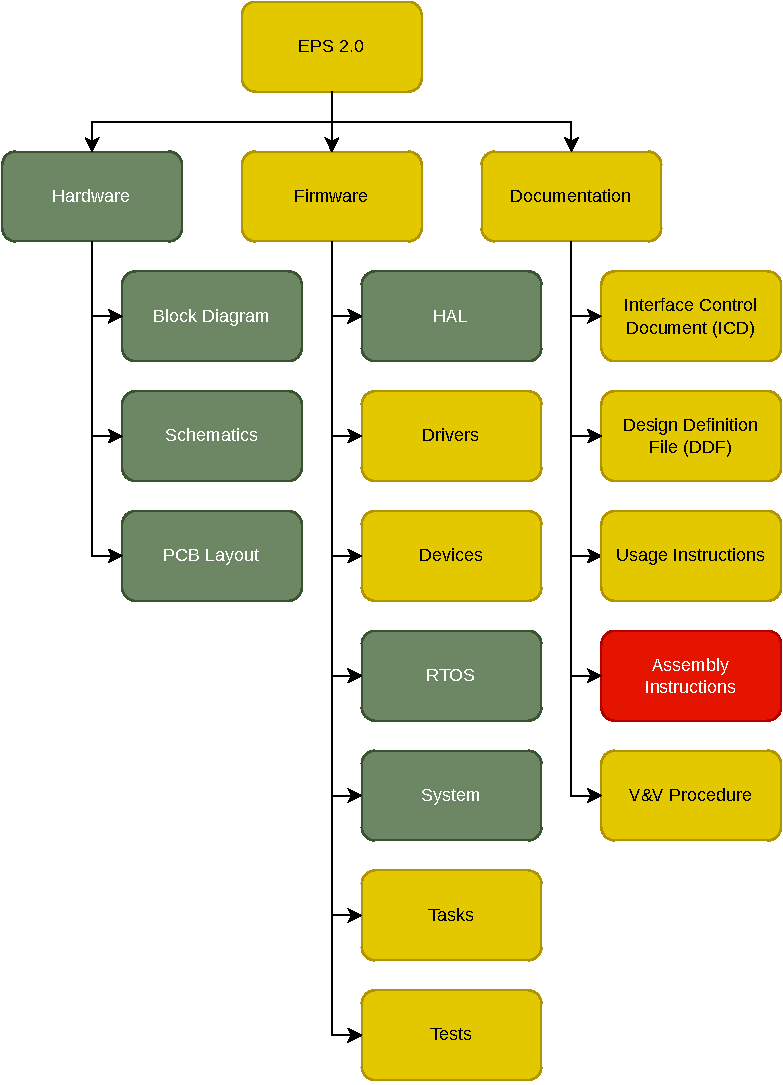
\includegraphics[width=0.8\textwidth]{figures/product-tree.pdf}
        \caption{Product tree of the EPS 2.0 module.}
        \label{fig:product-tree}
    \end{center}
\end{figure}

\section{MCU Block Diagram}

The \autoref{fig:mcu-block-diagram} presents a simplified view of the module subsystems and interfaces through the microcontroller perspective. 
The MCU has a programming JTAG\nomenclature{\textbf{JTAG}}{\textit{Joint Test Action Group.}}, a dedicated UART\nomenclature{\textbf{UART}}{\textit{Universal Asynchronous Receiver/Transmitter.}} debug interface and 4 communication buses, divided in 4 different protocols (I2C\nomenclature{\textbf{I2C}}{\textit{Inter-Integrated Circuit.}}, SPI\nomenclature{\textbf{SPI}}{\textit{Serial Peripheral Interface.}} and UART). 

There is an I2C buffer to allow secure and proper communication with the OBDH 2.0 module \cite{obdh2}.
The SPI protocol is used for controlling and retrieving data from an additional ADC\nomenclature{\textbf{ADC}}{\textit{Analog-to-Digital Converter.}} IC that measures temperature sensors (RTDs\nomenclature{\textbf{RTD}}{\textit{Resistance Temperature Detector.}}) on the batteries board and solar panels.
Several parameters from the Batteries Management Subsystem are sent to the EPS 2.0 MCU via I2C protocol.
The UART bus that goes to the PC/104 is used for basic telemetry to be sent to the beacon microcontroller within the TTC module.
Besides these channels, there are GPIO\nomenclature{\textbf{GPIO}}{\textit{General Purpose Input/Output.}} connections for enabling and disabling power buses, for hard code PCB versioning, and some optional GPIOs that can be added and used though the PC/104 interface. 

The MCU reads the measurements of current and voltage of the solar panels from its ADC ports for the MPPT Subsystem; also, from these data, the MPPT is controlled by the microcontroller through PWM\nomenclature{\textbf{PWM}}{\textit{Pulse Width Modulation.}} signals.

An external charger is used to charge the batteries and kill-switches to power off the EPS 2.0 module during the test phase. Before launch, the kill-switches are also connected to the button switches present on a CubeSat structure.   

\begin{figure}[!ht]
    \begin{center}
        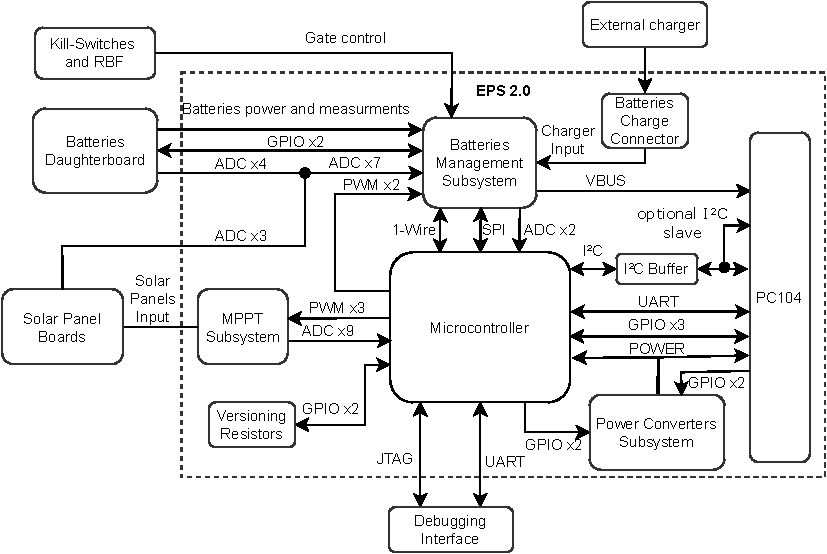
\includegraphics[width=0.75\textwidth]{figures/eps2_mcu_diagram.pdf}
        \caption{EPS 2.0 MCU Block diagram.}
        \label{fig:mcu-block-diagram}
    \end{center}
\end{figure}

\section{Power Block Diagram}

The \autoref{fig:power-block-diagram} presents a more detailed view of the power subsystems that complements the MCU Block Diagram. More details and descriptions about these hardware components and interfaces are provided in the \autoref{ch:hardware}.

\begin{figure}[!ht]
    \begin{center}
        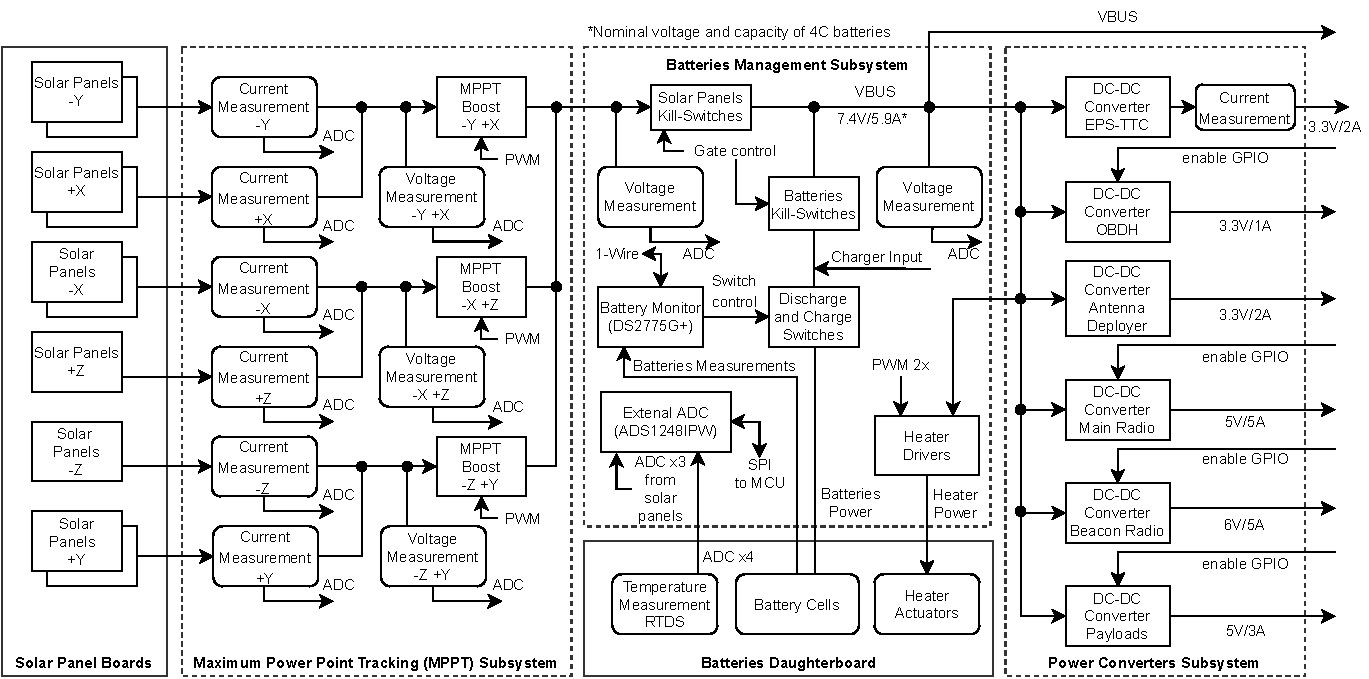
\includegraphics[width=\textwidth]{figures/eps2_power_diagram.pdf}
        \caption{EPS 2.0 Power Block diagram.}
        \label{fig:power-block-diagram}
    \end{center}
\end{figure}

\section{System Layers} \label{sec:system-layers}

The system is divided into various abstraction layers to favor high-level firmware implementations. The \autoref{fig:system-layers} shows this scheme, composed of third-party drivers at the lowest layer above the hardware, the operating system as the base building block of the module, the devices handling implementation, and the application tasks in the highest layer. More details are provided in the \autoref{ch:firmware}.

\begin{figure}[!ht]
    \begin{center}
        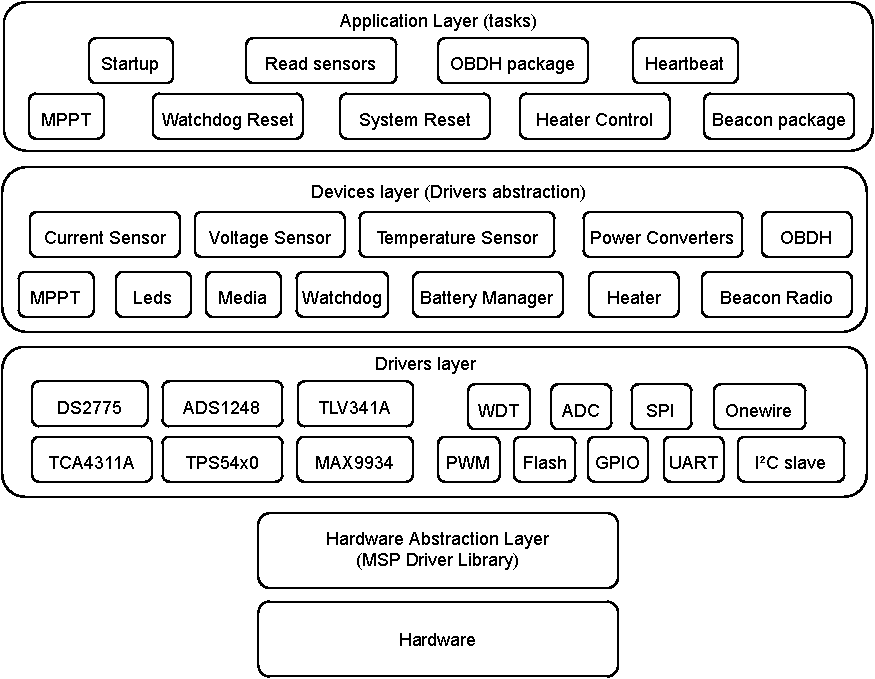
\includegraphics[width=0.75\textwidth]{figures/eps-system-layers.pdf}
        \caption{System layers.}
        \label{fig:system-layers}
    \end{center}
\end{figure}

\section{Operation} \label{sec:operation}

The system operates through the sequential execution of routines (tasks in the context of the operating system) that are scheduled and multiplexed through time. Each routine has a priority and a periodicity, determining the subsequent execution, the set of functionalities currently running, and the memory usage management.

Besides this deterministic scheduling system, the routines have communication channels with each other through the usage of queues, which provides a robust synchronization scheme. The system operation and internal nuances are described in detail in the \autoref{ch:firmware}. This section is a top view, user perspective, to describe the module's operation.

\subsection{Execution Flow}

To better understand how the EPS2 will operate during the mission, a simplified representation of its operation is presented in \autoref{fig:execution-flow}. Overall, the EPS2 should control the temperature of the battery and its energy harvesting system operation and obtain the sensors' measurements periodically. The OBDH or TTC modules can communicate with the EPS2, which should receive or transmit data as requested. Furthermore, every 10 hours, the EPS2 will reset.

\begin{figure}[!ht]
    \begin{center}
        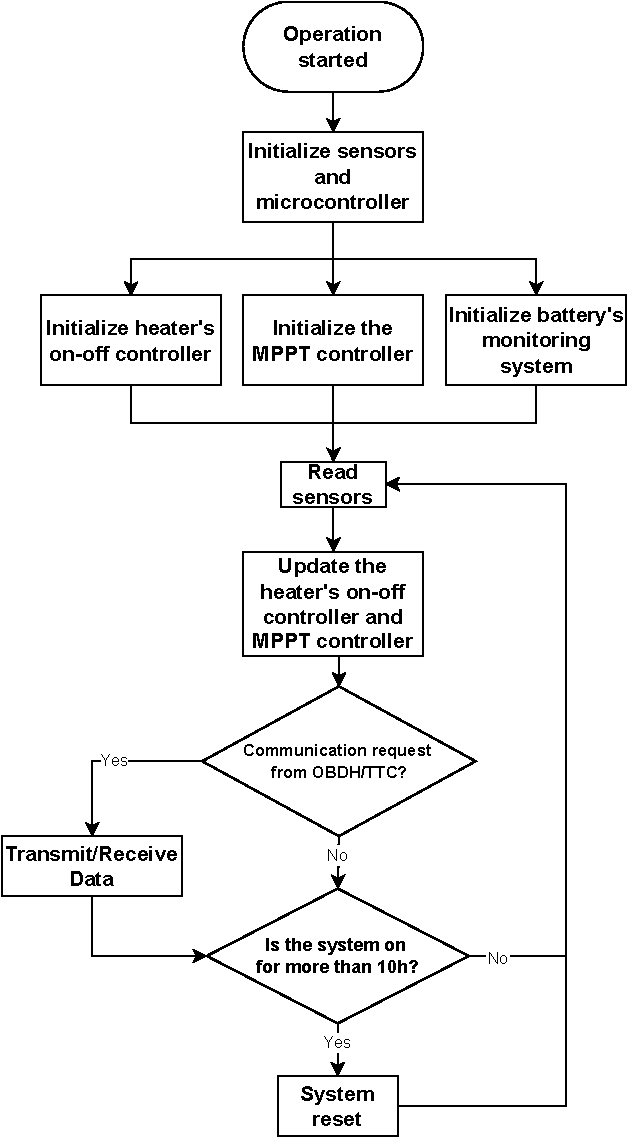
\includegraphics[width=0.5\textwidth]{figures/execution_flow.pdf}
        \caption{Simplified representation of the EPS2'S execution flow.}
        \label{fig:execution-flow}
    \end{center}
\end{figure}



%\subsection{Data Flow}
% Add here a flowchart or diagram showing where and how the data is generated and transferred across different modules and peripherals.

\subsection{Status LEDs} \label{status-leds}

On the development version of the board, there are ten LED\nomenclature{\textbf{LED}}{\textit{Light-Emitting Diode.}}s that indicate some behaviors of the systems. This set of LEDs can be seen on \autoref{fig:status-leds}.

\begin{figure}[!ht]
    \begin{center}
        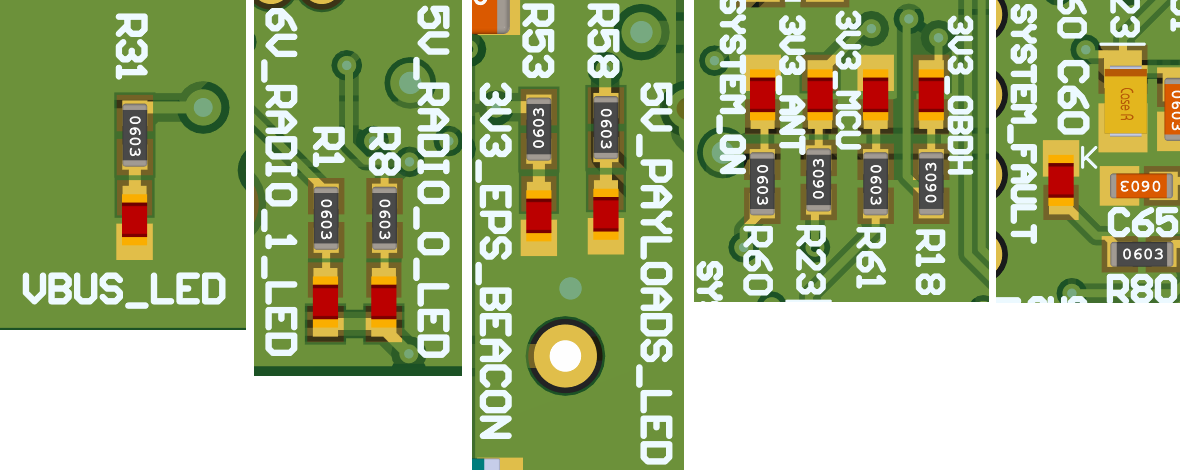
\includegraphics[width=\textwidth]{figures/status_leds.png}
        \caption{Available status LEDs.}
        \label{fig:status-leds}
    \end{center}
\end{figure}

A description of each of these LEDs is available below:

\begin{itemize}
    \item \textbf{6V\_RADIO\_1\_LED}: Indicates that the radio 1 transceiver 6V power is being sourced.
    \item \textbf{5V\_RADIO\_0\_LED}: Indicates that the radio 0 transceiver 5V power is being sourced.
    \item \textbf{SYSTEM\_ON}: Heartbeat of the system. It blinks at a frequency of 1 Hz when the system is running properly.
    \item \textbf{SYSTEM\_FAULT}: Indicates an error during the board's running firmware.
    \item \textbf{3V3\_ANT}: Indicates that the antenna deployer 3.3V power is being sourced.
    \item \textbf{3V3\_MCU}: Indicates that the EPS2 MCU 3.3V power is being sourced.
    \item \textbf{3V3\_OBDH}: Indicates that the OBDH module 3.3V power is being sourced.
    \item \textbf{3V3\_EPS\_BEACON}: Indicates that the EPS2 board and beacon MCU 3.3V power is being sourced.
    \item \textbf{5V\_PAYLOADS\_LEDS}: Indicates that the payloads 5V power is being sourced.
    \item \textbf{VBUS\_LED}: Indicates that the main power bus from the batteries is being sourced.
\end{itemize}

These LEDs are not mounted in the flight version of the module.

\section{Hard Code Versioning}

On the EPS2 board, there are 2 GPIOs dedicated to hard code versioning.
The on-board firmware can read these pins to identify the correct version of the hardware project.
Each line can be either pulled to VCC or ground, representing in binary as 1 and 0, respectively.
The \autoref{tab:versioning-resistors} shows the versioning representation up to the project's latest revision.

\begin{table}[!h]
    \centering
    \begin{tabular}{lcc}
        \toprule[1.5pt]
        \textbf{Version}    &   \textbf{P3.5 (pin code) / 47 (pin number)}    &    \textbf{P3.4 (pin code) / 46 (pin number)}\\
        \midrule
        v0.1                & 0                 & 0              \\
        v0.2                & 0                 & 1              \\
        \bottomrule[1.5pt]
    \end{tabular}
    \caption{Hard code versioning table.}
    \label{tab:versioning-resistors}
\end{table}

    %
% hardware.tex
%
% Copyright (C) 2021 by SpaceLab.
%
% EPS 2.0 Documentation
%
% This work is licensed under the Creative Commons Attribution-ShareAlike 4.0
% International License. To view a copy of this license,
% visit http://creativecommons.org/licenses/by-sa/4.0/.
%

%
% \brief Hardware project chapter.
%
% \author Gabriel Mariano Marcelino <gabriel.mm8@gmail.com>
% \author Yan Castro de Azeredo <yan.ufsceel@gmail.com>
%
% \institution Universidade Federal de Santa Catarina (UFSC)
%
% \version 0.1.1
%
% \date 2021/02/16
%

\chapter{Hardware} \label{ch:hardware}

The EPS2 is a 4 layer 1.6mm thick PCB with FR-4 dieletric. The module doesn't have any impedance control requirements, for this reason the layer stackup has 1oz (0.0347mm) thickness in inner and outer copper layers. In the following sections, the hardware design, interfaces, and standards are described in detail. Section are devided by subsystem blocks, following the diagrams present on \autoref{fig:mcu-block-diagram} and \autoref{fig:power-block-diagram}. The \autoref{fig:pcb-top}, \autoref{fig:pcb-bottom} and \autoref{fig:pcb-side} presents the 3D rendered images of the top, bottom and side views of the board, respectively.

\begin{figure}[!ht]
    \begin{center}
        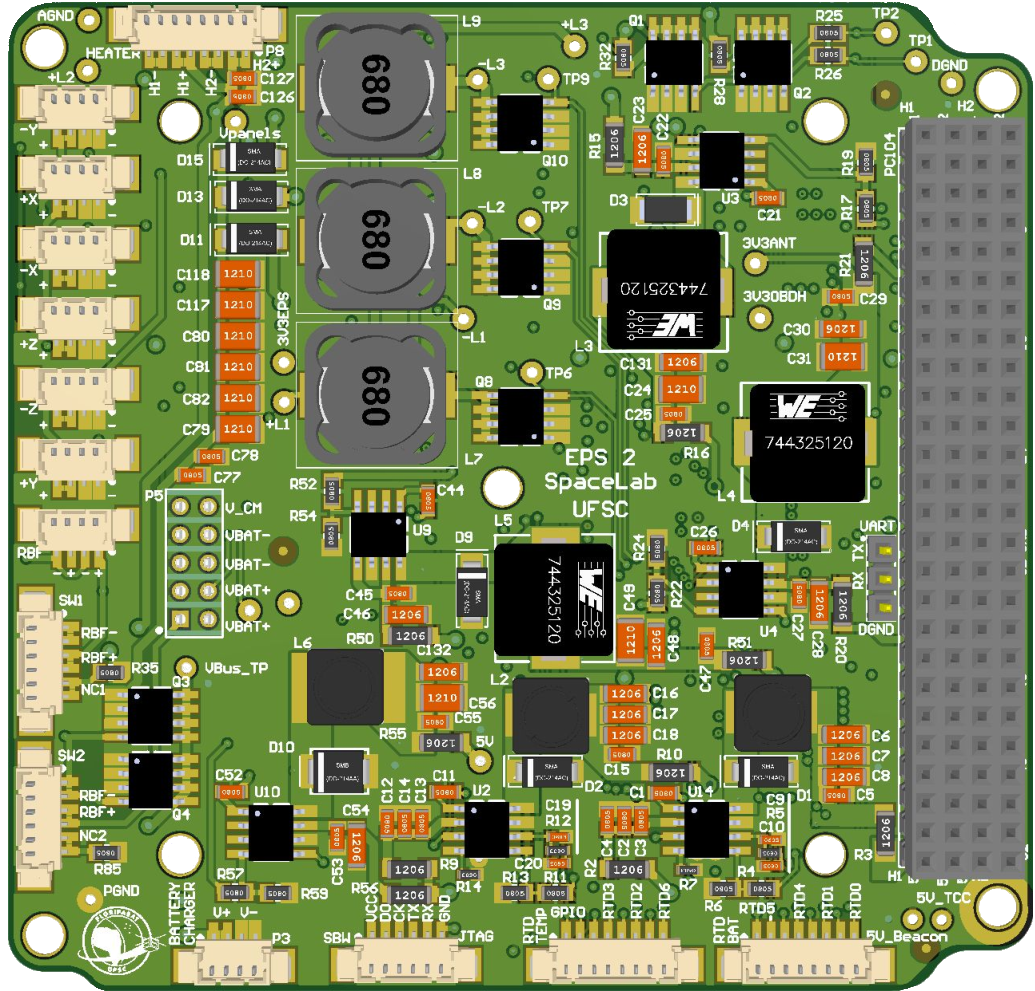
\includegraphics[width=93mm]{figures/eps2-pcb-top.png}
        \caption{Top side of the PCB.}
        \label{fig:pcb-top}
    \end{center}
\end{figure}

\begin{figure}[!ht]
    \begin{center}
        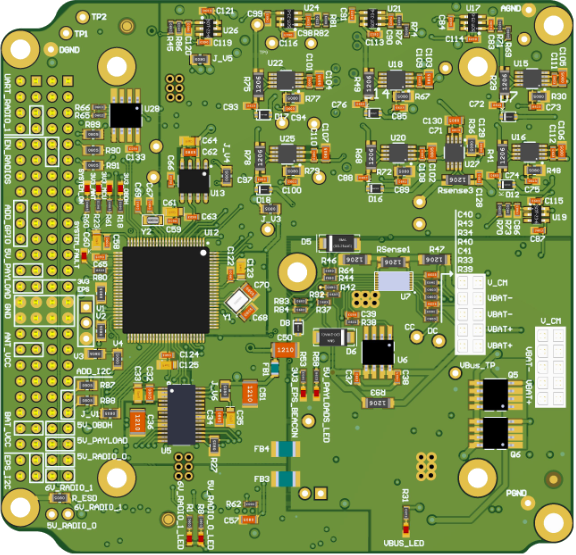
\includegraphics[width=93mm]{figures/eps2-pcb-bottom.png}
        \caption{Bottom side of the PCB.}
        \label{fig:pcb-bottom}
    \end{center}
\end{figure}

\begin{figure}[!ht]
    \begin{center}
        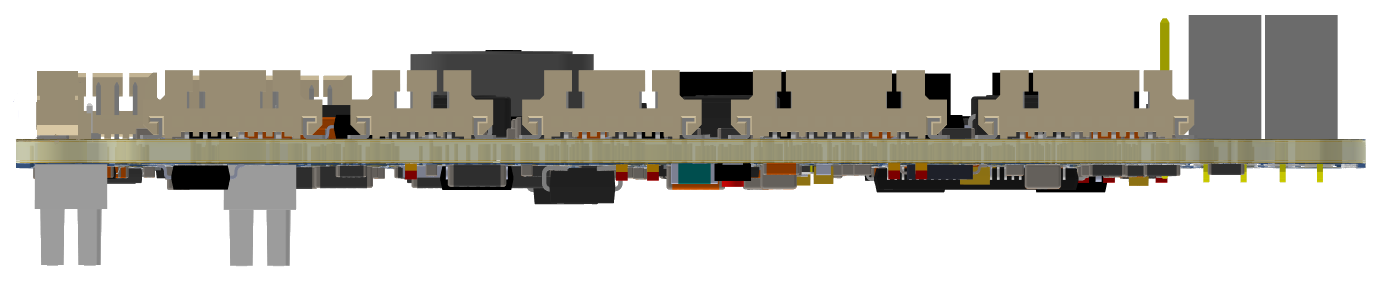
\includegraphics[width=93mm]{figures/eps2-pcb-side.png}
        \caption{Side view of the PCB.}
        \label{fig:pcb-side}
    \end{center}
\end{figure}

\section{Interfaces}

The \autoref{fig:diagram-interfaces} presents the board interfaces, which consists of communication with other modules, debug access points, and internal peripherals. From the perspective of the microcontroller, there are 4 individual communication buses and the JTAG interface (Spy-Bi-Wire), in the \autoref{tab:interfaces}: A1-SPI (dedicated for RTD analog readings with ADS1248); A0-UART (dedicated for Beacon Radio); A2-UART (dedicated for debug); B2-I2C (dedicated for OBDH); From the External Interface (IIP) can be acquired UART log messages for debbuging via USB without the use of an external UART to USB converter. The SPI comunicaton bus it actually an dedicated internall channel for the EPS MCU (master) to the ADS1248 (slave) ADC IC, the analog readings from BAT4C module (a.k.a Battery DaughterBoard) were also represented to show where the RTDs readings come from. \autoref{tab:usci-config} shows the interfaces configuration.

\begin{figure}[!ht]
    \begin{center}
        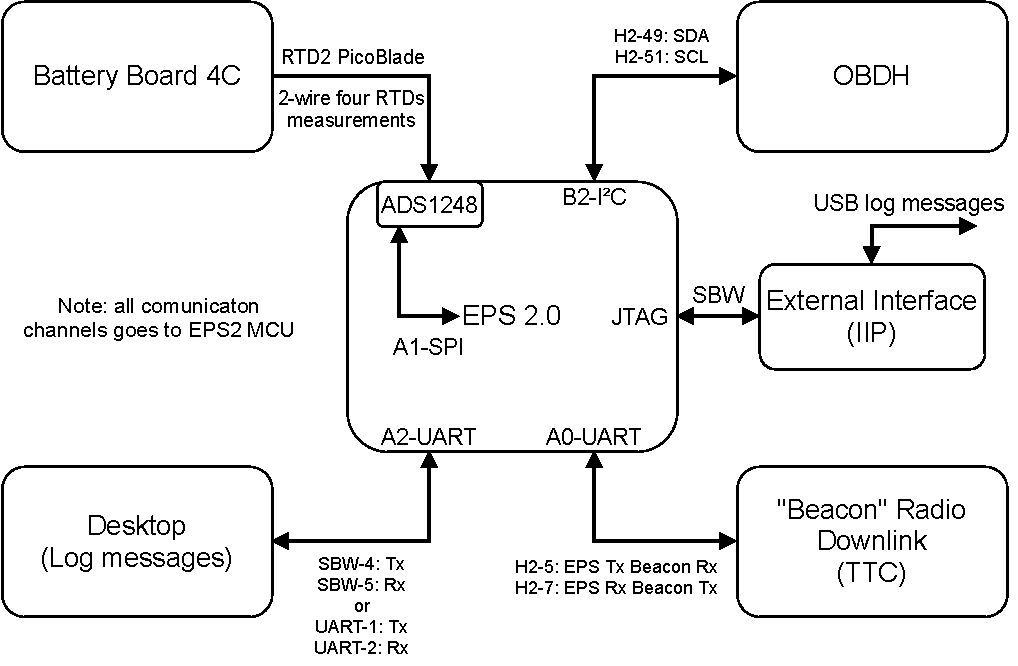
\includegraphics[width=\textwidth]{figures/eps-interfaces-diagram.pdf}
        \caption{EPS interfaces diagram.}
        \label{fig:diagram-interfaces}
    \end{center}
\end{figure}

\begin{table}[!h]
    \centering
    \begin{tabular}{lrrr}
        \toprule[1.5pt]
        \textbf{Peripheral}     & \textbf{USCI} & \textbf{Protocol} & \textbf{Comm. Protocol} \\
        \midrule
        ADS1248                 & A1            & SPI               & - \\
        Beacon Radio            & A0            & UART              & - \\
        PC (log messages)       & A2            & UART              & ANSI messages \\
        OBDH                    & B2            & I$^{2}$C          & FSP \\
        External Interface      & -             & JTAG              & Spy-Bi-Wire \\
        \bottomrule[1.5pt]
    \end{tabular}
    \caption{Boards interfaces.}
    \label{tab:interfaces}
\end{table}

\section{Microcontroller}

The MCU consists of a CPU, RAM Memory and Flash Memory (used for program storage and non-volatile status registers). The chosen MCU is a low power 16-bit RISC (\textit{MSP430F6659IPZR}) from Texas Instruments\cite{msp430f6659}. The \autoref{tab:msp430-summary} presents a summary of the main available features and \autoref{fig:msp430-diagram} shows the internal subsystems, descriptions, and peripherals. The microcontroller interfaces, configurations, and auxiliary components are described in the following topics.

\begin{table}[!h]
    \centering
    \begin{tabular}{cllllllll}
        \toprule[1.5pt]
        \textit{Flash} & \textit{SRAM} & \textit{Timers} & \textit{USCI} & \textit{ADC} & \textit{DAC} & \textit{GPIO} \\
        \midrule
        512KB  & 64KB  & 2  & 6 (SPI / I2C / UART)  & 12  & 2  & 74           \\
        \bottomrule[1.5pt]
    \end{tabular}
    \caption{Microcontroller features summary.}
    \label{tab:msp430-summary}
\end{table}

\begin{figure}[!ht]
    \begin{center}
        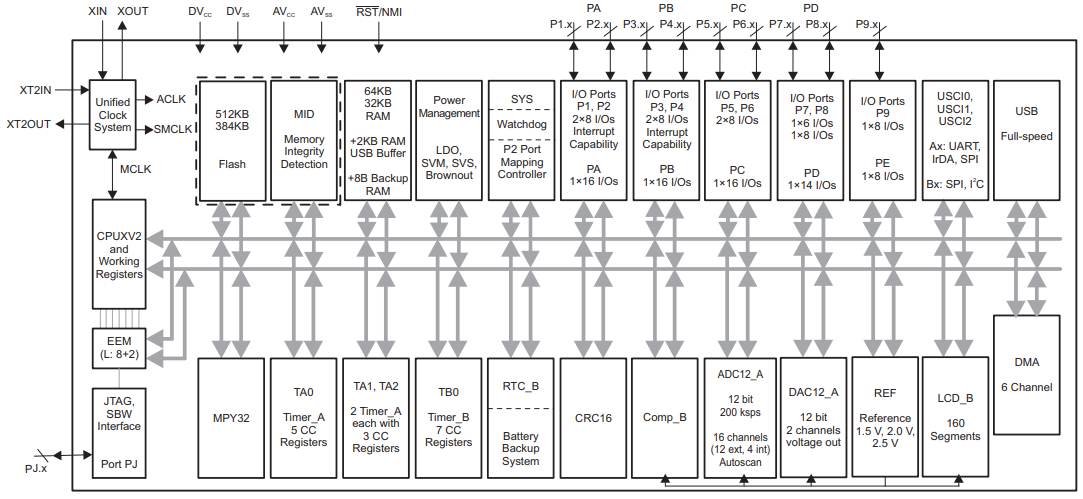
\includegraphics[width=\textwidth]{figures/msp430-diagram.png}
        \caption{Microcontroller internal diagram.}
        \label{fig:msp430-diagram}
    \end{center}
\end{figure}

\subsection{Interfaces Configuration}

The microcontroller has 6 Universal Serial Communication Interfaces (USCI) that can be configured to operate with different protocols and parameters. The \autoref{tab:usci-config} describes each interface configurations.

\begin{table}[!h]
    \centering
    \begin{tabular}{lrrrrl}
        \toprule[1.5pt]
        \textit{Interface} & \textit{Protocol (Index)} & \textit{Mode} & \textit{Word Length} & \textit{Data Rate} & \textit{Configuration} \\
        \midrule
        USCI\_A0           & UART0                     & -             & 8 bits               & 9600 bps           & Stop bits: 1 \\
                           &                           &               &                      &                    & Parity: None \\
        USCI\_A1           & SPI                       & Master        & 8 bits               & TBD                & Phase: High \\
                           &                           &               &                      &                    & Polarity: Low \\
        USCI\_A2           & UART1                     & -             & 8 bits               & 9600 bps           & Stop bits: 1 \\
                           &                           &               &                      &                    & Parity: None \\
        USCI\_B2           & I2C2                      & Slave         & 8 bits               & 100 kbps           & Address value: 0x36 \\
        \bottomrule[1.5pt]
    \end{tabular}
    \caption{USCI configuration.}
    \label{tab:usci-config}
\end{table}

\subsection{Voltage Reference}

To generate the 3 volts reference for the MCU internal ADC the EPS uses a \textit{595-REF5025AQDRQ1} chip.
Its circuit schematic can be seen in \autoref{fig:voltage-reference-circuit-schematic} and location on the PCB in \autoref{fig:voltage-reference-circuit-3d}.

\begin{figure}[!ht]
    \begin{center}
        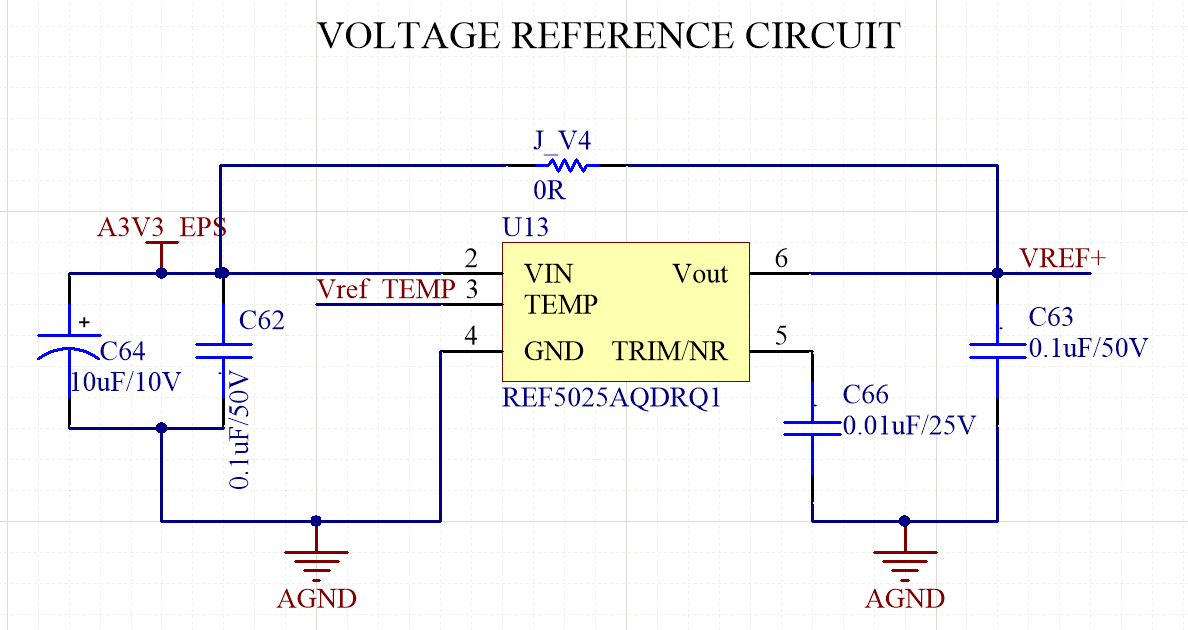
\includegraphics[width=0.8\textwidth]{figures/voltage-reference-circuit-schematic.png}
        \caption{Voltage reference circuit for EPS MCU schematic circuit.}
        \label{fig:voltage-reference-circuit-schematic}
    \end{center}
\end{figure}

\begin{figure}[!ht]
    \begin{center}
        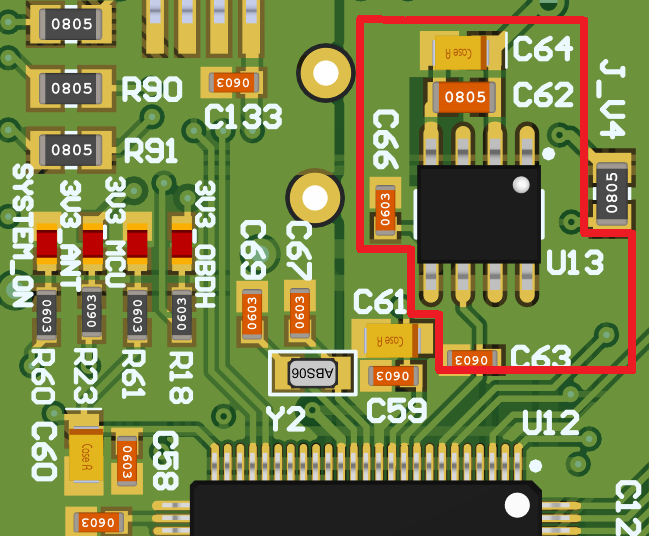
\includegraphics[width=0.5\textwidth]{figures/voltage-reference-circuit-3d.png}
        \caption{Voltage reference circuit for EPS MCU on the PCB.}
        \label{fig:voltage-reference-circuit-3d}
    \end{center}
\end{figure}

\subsection{Clocks Configuration}

Besides the internal clock sources, the microcontroller has two dedicated clock inputs for external crystals: the main clock and the auxiliary clock inputs. There are a 32MHz (\textit{ABM8X-102-32.000MHZ-T}) and a 32.769kHz (\textit{ECS-.327-12.5-34S-TR}) crystals connected to these inputs, respectively. The first source is used for generating the Master Clock (MCLK) and the Subsystem Master Clock (SMCLK), which are used by the CPU and the internal peripheral modules. The second source is used for generating the Auxiliary Clock (ACLK) that handles the low-power modes and might be used for peripherals.


\subsection{Pinout}

An illustration of the microcontroller pinout positions can be seen in the \autoref{fig:msp430-pinout-positions}. The \autoref{tab:mcu-pinout} presents all the EPS 2.0 microcontroller pins assignment.

\begin{figure}[!ht]
    \begin{center}
        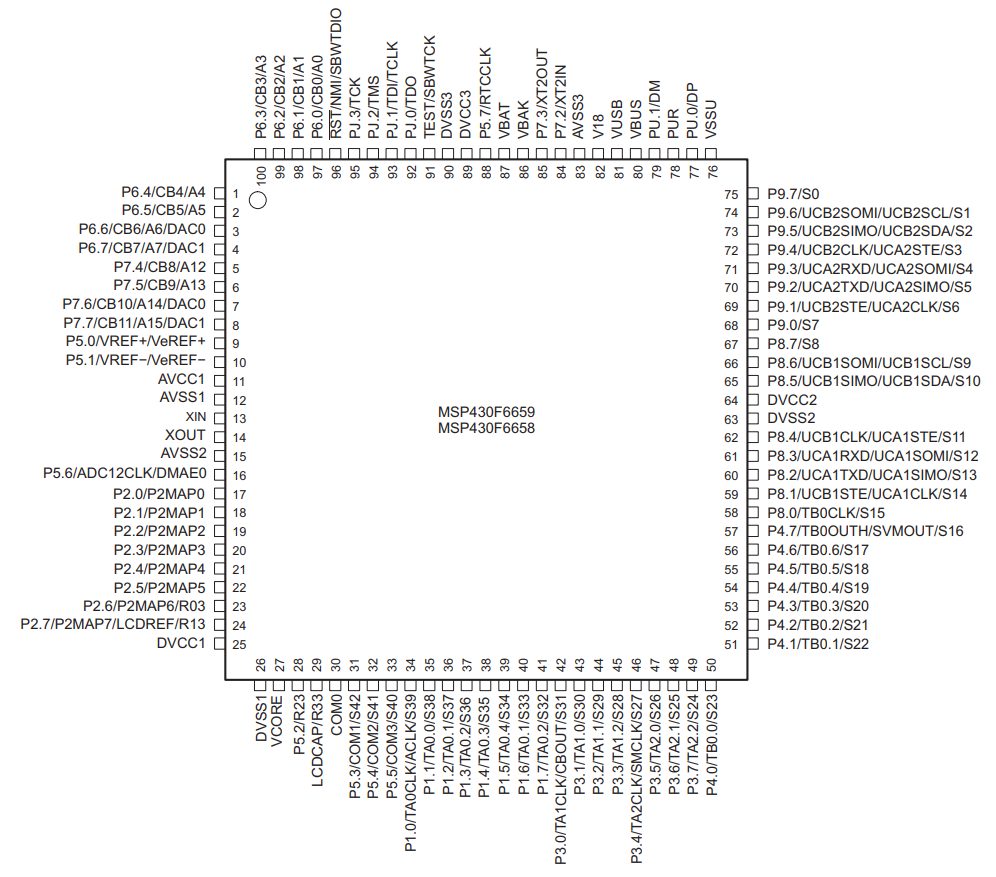
\includegraphics[width=0.9\textwidth]{figures/msp430-pinout.png}
        \caption{Microcontroller pinout positions.}
        \label{fig:msp430-pinout-positions}
    \end{center}
\end{figure}

\begin{longtable}{lcl}
    \toprule[1.5pt]
    \textit{Pin Code} & \textit{Pin Number} & \textit{Signal}       \\
    \midrule
    P1.0              & 34                  & -                 \\
    P1.1              & 35                  & -                 \\
    P1.2              & 36                  & EN\_3V3\_OBDH     \\
    P1.3              & 37                  & EN\_5V\_PAYLOADS  \\
    P1.4              & 38                  & -             \\
    P1.5              & 39                  & BAT\_GPIO1    \\
    P1.6              & 40                  & BAT\_GPIO2    \\
    P1.7              & 41                  & -             \\
    \midrule
    P2.0              & 17                  & -             \\
    P2.1              & 18                  & PC104\_GPIO0  \\
    P2.2              & 19                  & PC104\_GPIO1  \\
    P2.3              & 20                  & PC104\_GPIO2  \\
    P2.4              & 21                  & UART\_EPS\_TX\_BEACON\_RX     \\
    P2.5              & 22                  & UART\_EPS\_RX\_BEACON\_TX     \\
    P2.6              & 23                  & -                     \\
    P2.7              & 24                  & -                     \\
    \midrule
    P3.0              & 42                  & -                     \\
    P3.1              & 43                  & -                     \\
    P3.2              & 44                  & HEATER2\_PWM          \\
    P3.3              & 45                  & HEATER1\_PWM          \\
    P3.4              & 46                  & VERSION\_BIT0         \\
    P3.5              & 47                  & VERSION\_BIT1         \\
    P3.6              & 48                  & -                     \\
    P3.7              & 49                  & -                     \\
    \midrule
    P4.0              & 50                  & -                     \\
    P4.1              & 51                  & MPPT\_PWM\_1          \\
    P4.2              & 52                  & MPPT\_PWM\_2          \\
    P4.3              & 53                  & MPPT\_PWM\_3          \\
    P4.4              & 54                  & -                     \\
    P4.5              & 55                  & -                     \\
    P4.6              & 56                  & -                     \\
    P4.7              & 57                  & -                     \\
    \midrule
    P5.0              & 9                   & VREF                  \\
    P5.1              & 10                  & AGND                  \\
    P5.2              & 28                  & -                     \\
    P5.3              & 31                  & -                     \\
    P5.4              & 32                  & SYSTEM\_LED           \\
    P5.5              & 33                  & -                     \\
    P5.6              & 16                  & -                     \\
    P5.7              & 88                  & -                     \\
    \midrule
    P6.0              & 97                  & ADC1\_$+$Y\_SOLAR\_PANEL\_CURRENT \\
    P6.1              & 98                  & ADC2\_$+$X\_SOLAR\_PANEL\_CURRENT \\
    P6.2              & 99                  & ADC3\_$-$X\_SOLAR\_PANEL\_CURRENT \\
    P6.3              & 100                 & ADC4\_$+$Z\_SOLAR\_PANEL\_CURRENT \\
    P6.4              & 1                   & ADC5\_$-$Z\_SOLAR\_PANEL\_CURRENT \\
    P6.5              & 2                   & ADC6\_$+$Y\_SOLAR\_PANEL\_CURRENT \\
    P6.6              & 3                   & ADC7\_EPS\_TTC\_XCVR\_CURRENT \\
    P6.7              & 4                   & ADC\_MAIN\_POWER\_BUSS\_VOLTAGE \\
    \midrule
    P7.2              & 84                  & XT2\_N                \\
    P7.3              & 85                  & XT2\_P                \\
    P7.4              & 5                   & ADC1\_$-$Y\_$+$X\_SOLAR\_PANEL\_VOLTAGE \\
    P7.5              & 6                   & ADC2\_$-$X\_$+$Z\_SOLAR\_PANEL\_VOLTAGE \\
    P7.6              & 7                   & ADC3\_$-$Z\_$+$Y\_SOLAR\_PANEL\_VOLTAGE \\
    P7.7              & 8                   & ADC\_SOLAR\_PANELS\_TOTAL\_VOLTAGE \\
    \midrule
    P8.0              & 58                  & -                     \\
    P8.1              & 59                  & RTD\_SCLK             \\
    P8.2              & 60                  & RTD\_DIN              \\
    P8.3              & 61                  & RTD\_DOUT             \\
    P8.4              & 62                  & RTD\_RESET            \\
    P8.5              & 65                  & RTD\_CS               \\
    P8.6              & 66                  & RTD\_START            \\
    P8.7              & 67                  & RTD\_DRDY             \\
    \midrule
    P9.0              & 68                  & PIO                   \\
    P9.1              & 69                  & 1-WIRE                \\
    P9.2              & 70                  & UART0\_TX             \\
    P9.3              & 71                  & UART0\_RX             \\
    P9.4              & 72                  & I2C2\_EN              \\
    P9.5              & 73                  & I2C2\_SDA             \\
    P9.6              & 74                  & I2C2\_SCL             \\
    P9.7              & 75                  & I2C2\_READY           \\
    \midrule
    PJ.0              & 92                  & -                     \\
    PJ.1              & 93                  & -                     \\
    PJ.2              & 94                  & -                     \\
    PJ.3              & 95                  & -                     \\
    \midrule
    -                 & 13                  & XT1IN                 \\
    -                 & 14                  & XT1OUT                \\
    -                 & 96                  & JTAG\_TDO\_TDI        \\
    -                 & 91                  & JTAG\_TCK             \\
    \bottomrule[1.5pt]
    \caption{Microcontroller pinout and assignments.}
    \label{tab:mcu-pinout}
\end{longtable}

\section{Batteries DaughterBoard}

Due to size restrictions the 4 cell batteries of the EPS2 were allocated to a dauhterboard named Battery Module 4 Cells, a.k.a BAT4C\nomenclature{\textbf{BAT4C}}{\textit{Battery Module 4 Cells.}}\cite{bat4c}. Both boards 3D models are assembled together in a EDA tool as seen in \autoref{fig:eps2-pcb-3d-battery}. BAT4C is connected below EPS2 in a board-to-board connector, the female counterpart (\textit{BAT4CIPS1-105-01-S-D}) present on the EPS is seen in \autoref{fig:battery-connector} with it pinout present on \autoref{tab:battery-connector}. For compability with the older version of the battery module the same connector pads are present near the middle section of the PCB. If the BAT4C is to be used, the connector for these pads must not be soldered, more detail on \autoref{ch:assembly}. Also external connectors are used for temperature measurement and control with RTDs and heaters, more details can be seen on \autoref{rtd-picoblade} and \autoref{heater-picoblade}. 

\begin{figure}[!ht]
    \begin{center}
        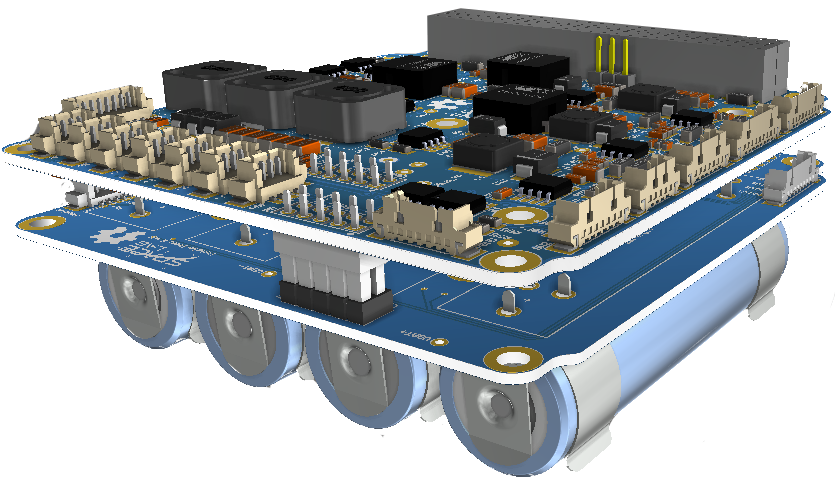
\includegraphics[width=93mm]{figures/eps2-pcb-3d-battery.png}
        \caption{EPS2 and BAT4C 3D models assembled.}
        \label{fig:eps2-pcb-3d-battery}
    \end{center}
\end{figure}

\begin{figure}[!ht]
    \begin{center}
        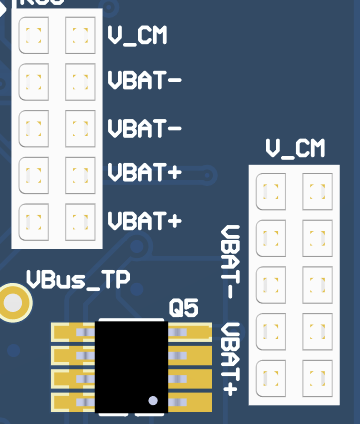
\includegraphics[width=0.35\textwidth]{figures/battery-connector.png}
        \caption{EPS2 battery connectors.}
        \label{fig:battery-connector}
    \end{center}
\end{figure}

\begin{table}[!h]
    \centering
    \begin{tabular}{cllll}
        \toprule[1.5pt]
        \textit{Pin} & \textit{Row} \\
        \midrule
        1            & $+$Vbat \\
        2            & $+$Vbat \\
        3            & $+$Vbat \\
        4            & $+$Vbat \\
        5            & $-$Vbat \\
        6            & $-$Vbat \\
        7            & $-$Vbat \\
        8            & $-$Vbat \\
        9            & Vbat\_Common \\
        10           & Vbat\_Common \\
        \bottomrule[1.5pt]
    \end{tabular}
    \caption{Battery connector pinout.}
    \label{tab:battery-connector}
\end{table}

\section{Solar Panels}

The energy harvesting system is based on solar energy conversion through ten solar panels attached to a 2U CubeSat structure. The solar panels are connected through six 4 pin PicoBlade connectors \textit{0533980471}. Because the EPS2 module has only six input connectors four pairs of solar panels will be connected in paralel. The connection scheme of the solar panels is visible in \autoref{fig:diagram-solar-panels}. The input connectors for the solar panels power are described in \autoref{solar-panels-picoblades}.
\begin{figure}[!ht]
    \begin{center}
        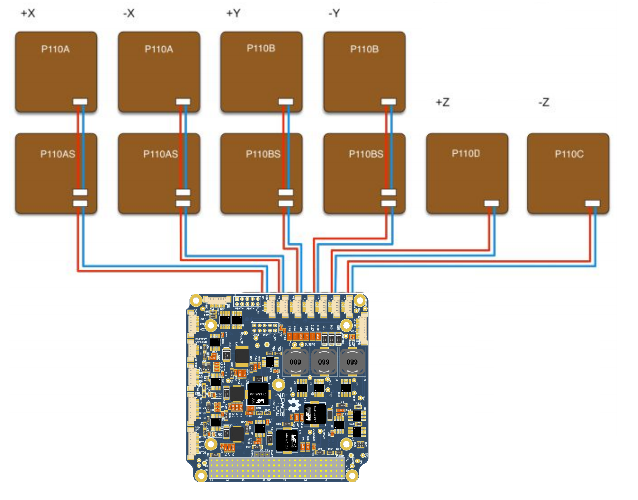
\includegraphics[width=0.75\textwidth]{figures/diagram-solar-panels.png}
        \caption{Solar panels connection to EPS2.}
        \label{fig:diagram-solar-panels}
    \end{center}
\end{figure}

\section{I2C Buffer}

The microcontroller I2C interface have a dedicated IC buffer, which improve the signal quality throughout the various connectors and offers reliability enhancements, since it protects the bus in case of failures. This measure was adopted in all the satellite modules due to previous failures in I2C buses. Using this scheme, the modules connected though this protocol might have shared connections without losing performance or reliability. 

The buffer selected for this function is the Texas Instruments \textit{TCA4311}. Besides the I2C inputs and outputs, it features control and status signals that are connected to GPIOs in the microcontroller: an enable and an operation ready status. Also, both inputs and outputs in these I2C lines have external pull-up resistors. Its circuit schematic can be see \autoref{fig:i2c-buffer-circuit}.

\begin{figure}[!ht]
    \begin{center}
        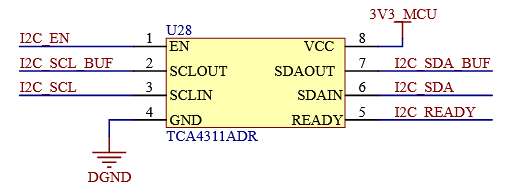
\includegraphics[width=0.65\textwidth]{figures/i2c-buffer-circuit.png}
        \caption{I2C buffer circuit.}
        \label{fig:i2c-buffer-circuit}
    \end{center}
\end{figure}

\section{MPPT Subsystem}

On the MPPT subsystem the main components are the MPPT boost converters, solar panels voltage and current sensors. These measurement circuits are used to generate a voltage proportional to the variable being measured, in a range accepted by the MCU internal ADC.

\subsection{MPPT Boost Converters}

There are three boost converters in the system, one for each couple of solar panels in parallel connection. Each one is a discrete boost with a \textit{HC9-220-R} inductor, a \textit{SI4166DY} mosfet as the switch and a \textit{B340LA-13-F} diode. There are six \textit{GRM32ER1E226KE15L} capacitors and two \textit{GRM216R71H103KA01D} capacitors connected in parallel in the boost output. The output filter is the same for all the converters as their outputs are tied together. The control PWM signals are generated by the MCU at a frequency of nearly 500 kHz.
One of the MPPT boosters circuit schematic can be seen in \autoref{fig:mppt-boosters-circuit-schematic} and location of all three at the PCB in \autoref{fig:mppt-boosters-circuit-3d}.

\begin{figure}[!ht]
    \begin{center}
        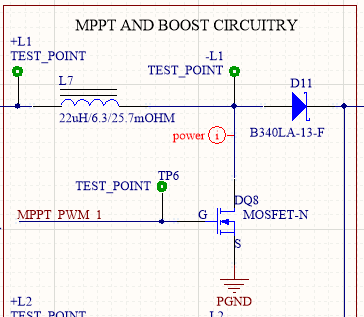
\includegraphics[width=0.5\textwidth]{figures/mppt-boosters-circuit-schematic.png}
        \caption{One of the MPPT boosters schematic circuit.}
        \label{fig:mppt-boosters-circuit-schematic}
    \end{center}
\end{figure}

\begin{figure}[!ht]
    \begin{center}
        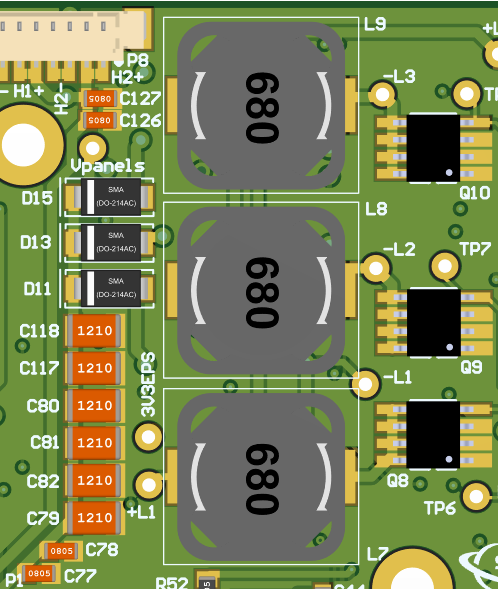
\includegraphics[width=0.5\textwidth]{figures/mppt-boosters-circuit-3d.png}
        \caption{MPPT boost converters circuit on the PCB.}
        \label{fig:mppt-boosters-circuit-3d}
    \end{center}
\end{figure}

\subsection{Solar Panels Current}

The main component of the solar panels currents measurement circuit is the \textit{MAX9934TAUA+} current sense amplifier. It generates an output current proportional to the differential input voltage. The gain is 25 $\mu$A/mV. To make the measurements possible, the current goes through 50 m$\Omega$, 0.5 \% resistors, connected to the inputs of the amplifier, and the outputs are connected to 3.3 k$\Omega$ resistors. The output voltage of the circuit is given by:

\begin{equation}
V_{out} = I_{sense} \cdot R_{sense} \cdot G \cdot R_{out}
\end{equation}

In total there are six of these current measurement circuits for the six sides of the CubeSat.
Two of the inputs of the solar panels circuit schematic can be seen in \autoref{fig:solar-panels-current-circuit-schematic} and location of all six at the PCB in \autoref{fig:solar-panels-current-circuit-3d}.

\begin{figure}[!ht]
    \begin{center}
        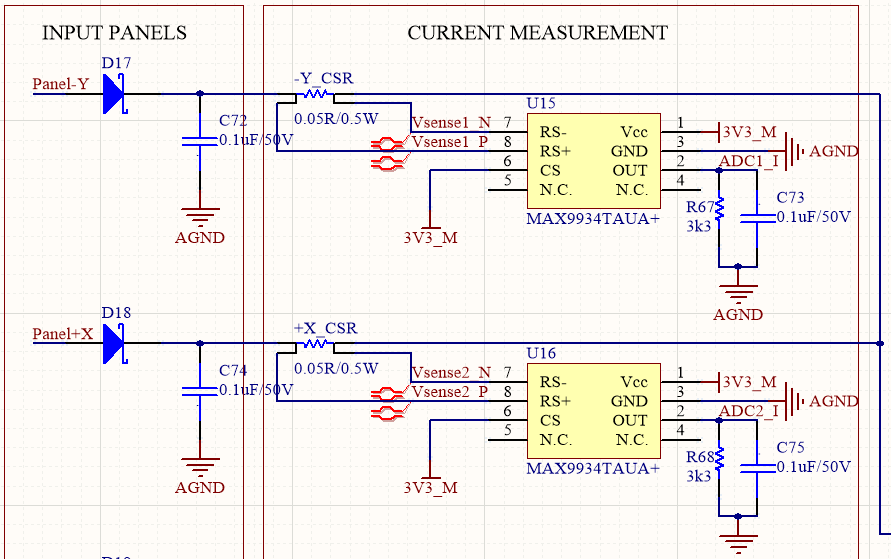
\includegraphics[width=0.85\textwidth]{figures/solar-panels-current-circuit-schematic.png}
        \caption{Solar panels $-$Y and $+$X input circuit schematic.}
        \label{fig:solar-panels-current-circuit-schematic}
    \end{center}
\end{figure}

\begin{figure}[!ht]
    \begin{center}
        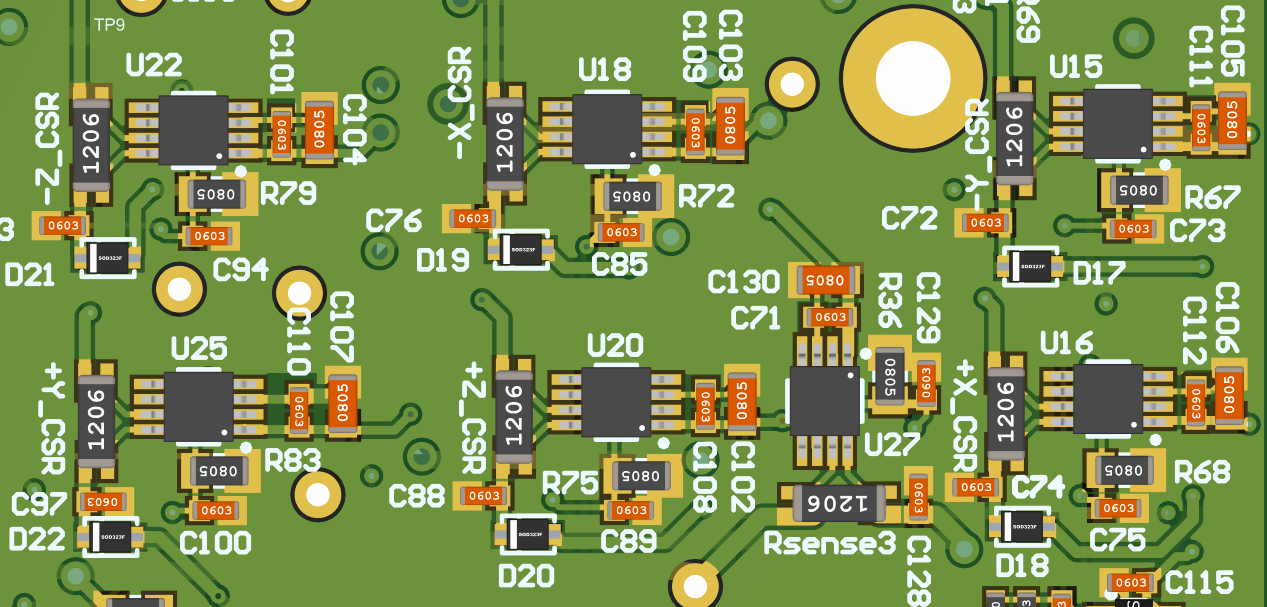
\includegraphics[width=0.85\textwidth]{figures/solar-panels-current-circuit-3d.png}
        \caption{Solar panels current measurement circuits on the PCB.}
        \label{fig:solar-panels-current-circuit-3d}
    \end{center}
\end{figure}


\subsection{Solar Panels Voltage}

The solar panels voltage measurement circuit is composed by a voltage divider and an op-amp in a buffer configuration. The voltage divider is composed of a 93.1 k$\Omega$ resistor and an 100 k$\Omega$ resistor. The op-amp is a \textit{TLV341AIDBVR} chip. The output voltage is given by:

\begin{equation}
V_{out} = V_{sp} \cdot \frac{R_{2}}{R_{1} + R_{2}}
\end{equation}

In total there are three of these voltage measurement circuits, the solar panels sides that are meassured together are: $-$Y with $+$X, $-$X with $+$Z and $-$Z with $+$Y.
One of the voltage measurement circuit schematic can be seen in \autoref{fig:solar-panels-voltage-circuit-schematic}.

\begin{figure}[!ht]
    \begin{center}
        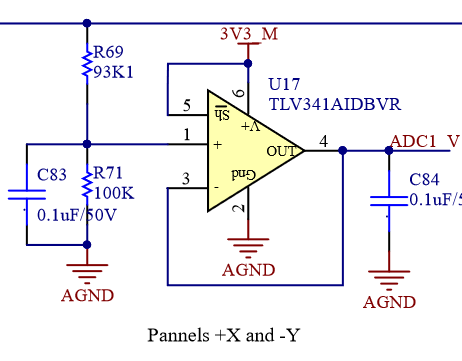
\includegraphics[width=0.5\textwidth]{figures/solar-panels-voltage-circuit-schematic}
        \caption{Solar panels $-$Y and $+$X voltage measurement circuit schematic.}
        \label{fig:solar-panels-voltage-circuit-schematic}
    \end{center}
\end{figure}

\section{Batteries Managment Subsystem}

On the batteries managment subsystem the main components are the battery control circuit, external ADC chip, solar panels and batteries kill-switches, heater drivers and voltage sensors for the boosters output and main power bus. 

\subsection{Boost Converters Output Voltage}

The boost converters output voltage measurement circuit is very similar to the solar panels voltages measurement circuit, with the exception that the voltage divider is composed by a 300 k$\Omega$ resistor and an 100 k$\Omega$ resistor.
The schematic for the voltage measurement circuit of the solar panels can be seen again for reference in \autoref{fig:solar-panels-voltage-circuit-schematic}.

\subsection{Kill-Switches and Remove Before Flight}

These switches are used to separate the solar panels and the batteries from the load during pre-flight and launch. Each one is composed of two \textit{SI4403-CDY-T1-GE3} P-channel mosfets in parallel, as a redundancy.
The Kill-Switches and RBF\nomenclature{\textbf{RBF}}{\textit{Remove Before Flight.}} are interfaced on the EPS board via external PicoBlade cables to its respective external mechanisms. RBF functions by simply short circuting the pins of the pin header present on an external interface\cite{iip}, and for the kill-switches it is required to press the spring buttons on the CubeSat structure, this is naturally done when the nanosatellite in integrated into the deployer.
On \autoref{kill-switches-picoblades} and \autoref{rbf-picoblade} it is showed the pinouts and locations for these connectors.

\subsection{Battery Control Circuit}

The batteries are monitored by the \textit{DS2775} chip. It measures several parameters and sends them to the EPS2 MCU via one-wire protocol. Also it automatically protects the batteries against short-circuits, overvoltage and undervoltage situations by switching two \textit{FDS6898AZ} mosfets.
Its circuit schematic can be seen in \autoref{fig:bms-circuit-schematic} and location on the PCB in \autoref{fig:bms-circuit-3d}.

\begin{figure}[!ht]
    \begin{center}
        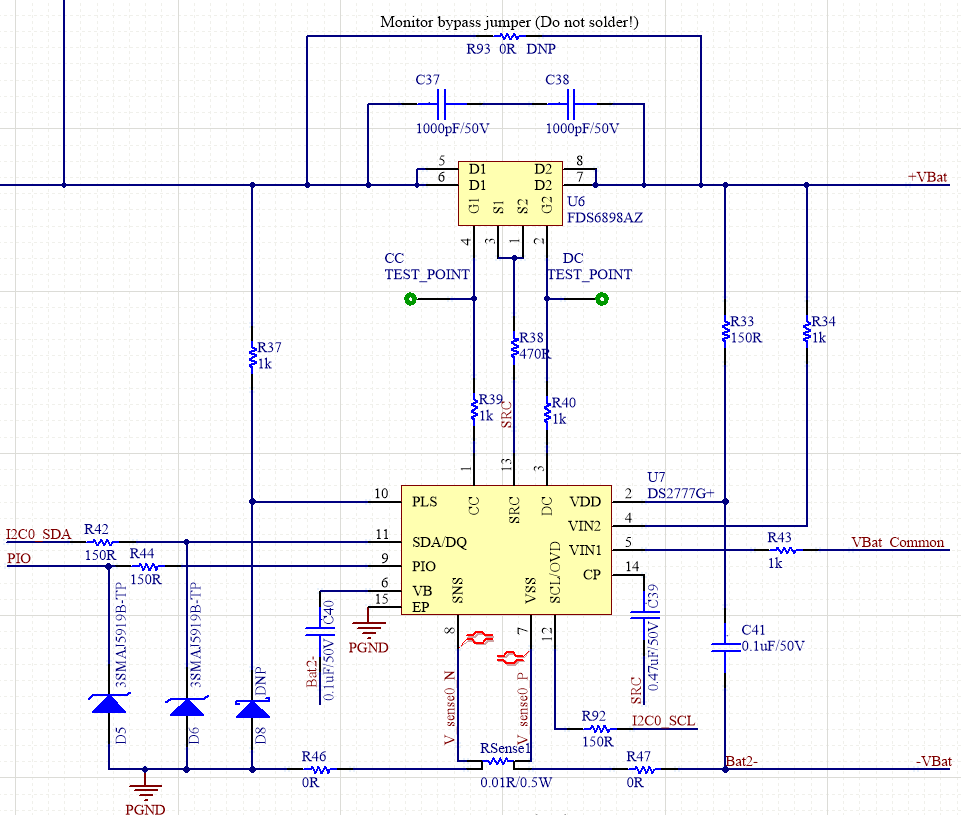
\includegraphics[width=\textwidth]{figures/bms-circuit-schematic.png}
        \caption{Battery monitor circuit schematic.}
        \label{fig:bms-circuit-schematic}
    \end{center}
\end{figure}

\begin{figure}[!ht]
    \begin{center}
        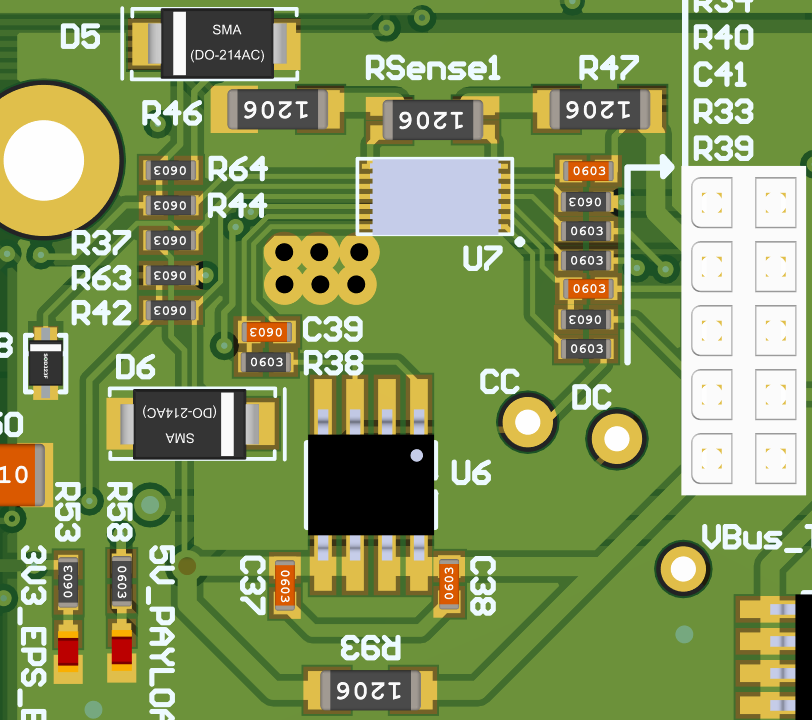
\includegraphics[width=0.5\textwidth]{figures/bms-circuit-3d.png}
        \caption{Battery monitor circuit on the PCB.}
        \label{fig:bms-circuit-3d}
    \end{center}
\end{figure}

\subsection{Main Power Bus Voltage}

The main power bus voltage measurement circuit is identical to the boost converters output voltage measurement circuit.
The schematic for the voltage measurement circuit of the solar panels can be seen again for reference in \autoref{fig:solar-panels-voltage-circuit-schematic}.

\subsection{External ADC}

The \textit{ADS1248} chip generates a precise reference current to the RTDs, and samples the voltage proportional to the temperature established over the sensors. This voltage is converted to digital data and sent to the MCU via SPI protocol.
The location the IC and its subcircuitry can be seen in \autoref{fig:ads1248-circuit-3d}.

\begin{figure}[!ht]
    \begin{center}
        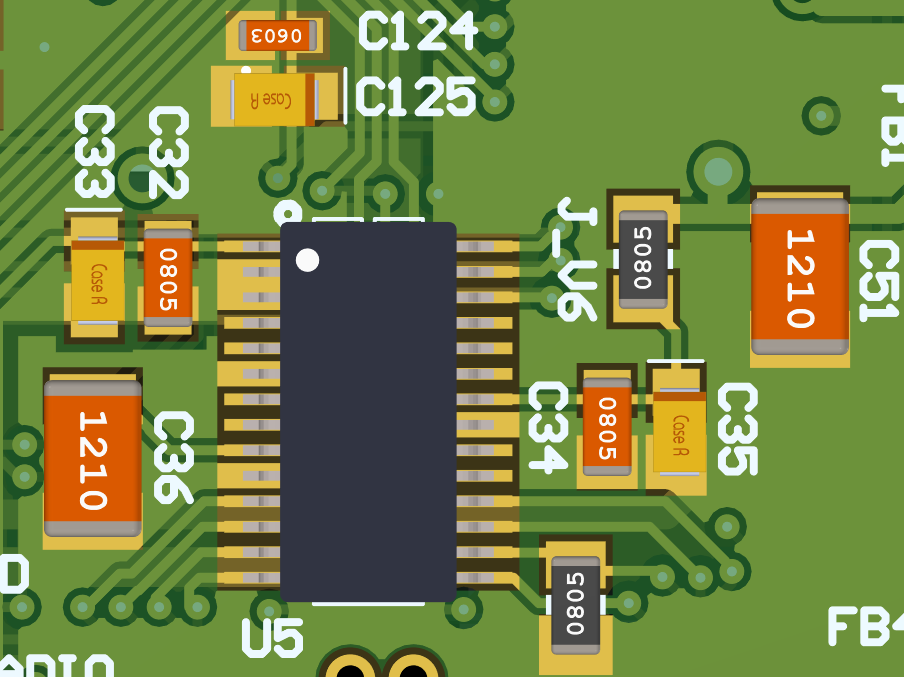
\includegraphics[width=0.5\textwidth]{figures/ads1248-circuit-3d.png}
        \caption{ADS1248 circuit on the PCB.}
        \label{fig:ads1248-circuit-3d}
    \end{center}
\end{figure}

\subsection{Heaters Drivers}

The drivers are chopper converters controlled by the MCU, with a PWM frequency of 50 kHz. The switches of the chopper converters are \textit{Si4010DY} mosfets.
Its circuit schematic can be seen in \autoref{fig:heaters-circuit-schematic} and location on the PCB in \autoref{fig:heaters-drivers-circuit-3d}.

\begin{figure}[!ht]
    \begin{center}
        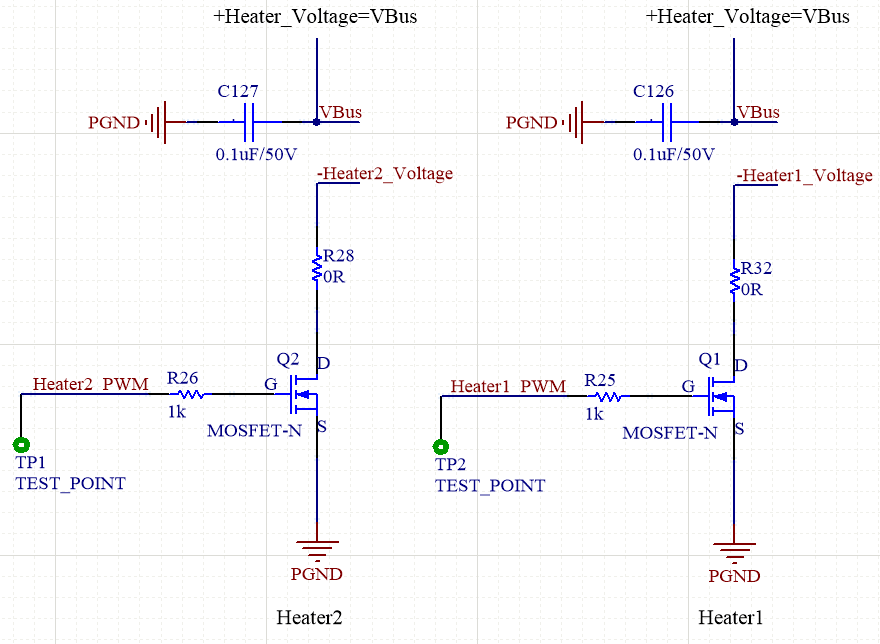
\includegraphics[width=\textwidth]{figures/heaters-drivers-circuit-schematic.png}
        \caption{Hearter drivers circuit schematic.}
        \label{fig:heaters-circuit-schematic}
    \end{center}
\end{figure}

\begin{figure}[!ht]
    \begin{center}
        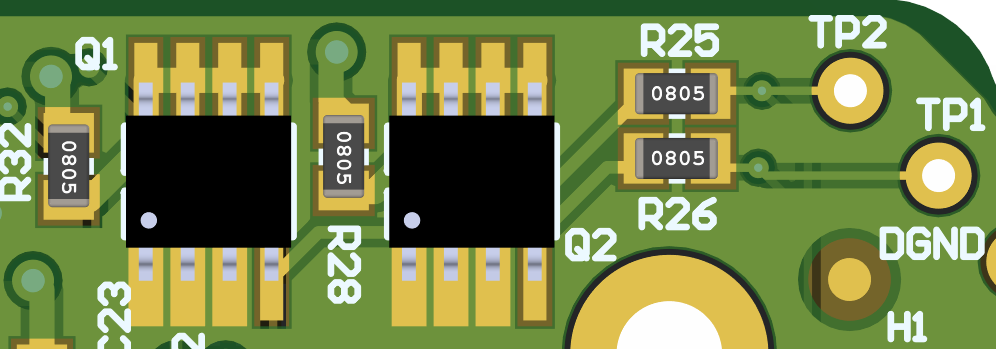
\includegraphics[width=0.5\textwidth]{figures/heaters-drivers-circuit-3d.png}
        \caption{Hearter drivers circuit on the PCB.}
        \label{fig:heaters-drivers-circuit-3d}
    \end{center}
\end{figure}

\section{Power Converters Subsystem}

The EPS2 has 6 integrated buck DC-DC regulators, all these are powered from the main power bus. Some regulators are always enabled, others are can be enabled or disabled by the EPS2 or other module.

\subsection{EPS/TTC Regulator}

To supply the TTC MCU (also called "Beacon MCU") and EPS2 MCU and its subcircuits a \textit{TPS5420QDRQ1} regulator is used, with and output voltage of 3.3 V and 2 A current capability. This regulator is always on.
The EPS/TTC circuit location on the PCB can be seen in \autoref{fig:eps-beacon-buck-circuit-3d}.

\begin{figure}[!ht]
    \begin{center}
        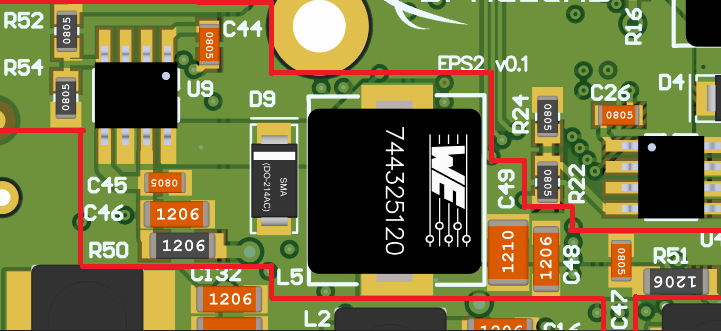
\includegraphics[width=0.5\textwidth]{figures/eps-beacon-buck-circuit-3d.png}
        \caption{EPS/TTC regulator circuit on the PCB.}
        \label{fig:eps-beacon-buck-circuit-3d}
    \end{center}
\end{figure}

There is also a current measurement at the output of the EPS/TTC regulator. It also uses a \textit{MAX9934TAUA+} current sense amplifier, but with a shunt resistor of 75 m$\Omega$, 0.5 \% and the output connected to a 4.02 k$\Omega$ resistor.
The circuit schematic is almost the same as \autoref{fig:solar-panels-current-circuit-schematic} only changing the resistors and capacitor values, its location on the PCB is the labeled U27 IC and its passive components in \autoref{fig:solar-panels-current-circuit-3d}.

\subsection{OBDH Regulator}

The OBDH is powered by a \textit{TPS5410QDRQ1} regulator, with an output voltage of 3.3 V and 1 A current capability. The EPS2 can enable/disable this regulator.
Its location on the PCB can be seen in \autoref{fig:obdh-buck-circuit-3d}.

\begin{figure}[!ht]
    \begin{center}
        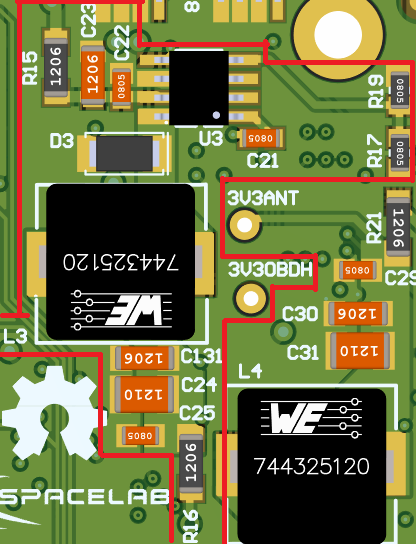
\includegraphics[width=0.3\textwidth]{figures/obdh-buck-circuit-3d.png}
        \caption{OBDH regulator circuit on the PCB.}
        \label{fig:obdh-buck-circuit-3d}
    \end{center}
\end{figure}

\subsection{Antenna Deployer Regulator}

The antenna deployment system has a dedicated regulator \textit{TPS5420QDRQ1}, with 3.3 V output voltage and 2 A current capability. This regulator is always on.
Its location on the PCB can be seen in \autoref{fig:ant-buck-circuit-3d}.

\begin{figure}[!ht]
    \begin{center}
        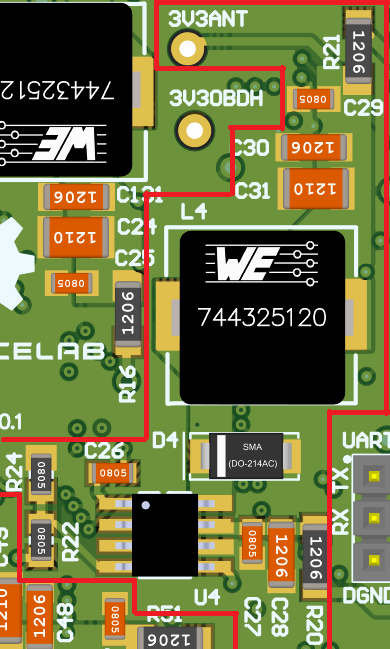
\includegraphics[width=0.3\textwidth]{figures/ant-buck-circuit-3d.png}
        \caption{Antenna deployer regulator circuit on the PCB.}
        \label{fig:ant-buck-circuit-3d}
    \end{center}
\end{figure}

\subsection{Main Radio Transceiver Regulator}

The main radio XCVR\nomenclature{\textbf{XCVR}}{\textit{Transceiver.}} responsible for the Downlink/Uplink of the CubeSat is powered by a \textit{TPS54540QDDARQ1} regulator, with an output voltage of 5V and 5A campability. The OBDH can enable/disable this regulator.
Its location on the PCB can be seen in \autoref{fig:main-radio-buck-circuit-3d}.

\begin{figure}[!ht]
    \begin{center}
        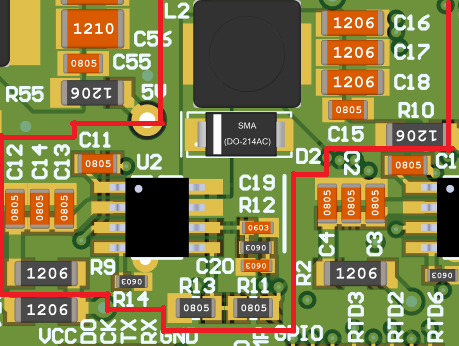
\includegraphics[width=0.5\textwidth]{figures/main-radio-buck-circuit-3d.png}
        \caption{Main radio transceiver regulator circuit on the PCB.}
        \label{fig:main-radio-buck-circuit-3d}
    \end{center}
\end{figure}

\subsection{Beacon Transceiver Regulator}

The Beacon XCVR is powered by a regulator \textit{TPS54540QDDARQ1} regulator, with 6V output voltage and 5A campability. The Beacon MCU can enable/disable this regulator.
Its location on the PCB can be seen in \autoref{fig:beacon-radio-buck-circuit-3d}.

\begin{figure}[!ht]
    \begin{center}
        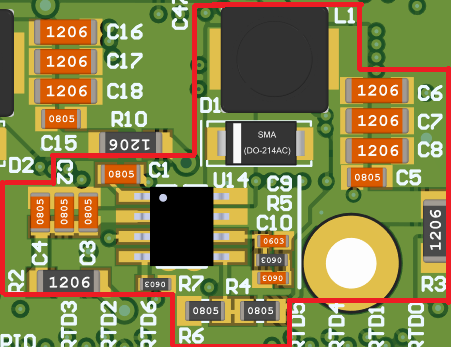
\includegraphics[width=0.5\textwidth]{figures/beacon-radio-buck-circuit-3d.png}
        \caption{Beacon radio transceiver regulator circuit on the PCB.}
        \label{fig:beacon-radio-buck-circuit-3d}
    \end{center}
\end{figure}

\subsection{Payloads Regulator}

To power the payloads a \textit{TPS5430QDDARQ1} regulator is used. It has an output voltage of 5 V and 3 A current capability. The EPS2 can enable/disable this regulator.
Its location on the PCB can be seen in \autoref{fig:payloads-buck-circuit-3d}.

\begin{figure}[!ht]
    \begin{center}
        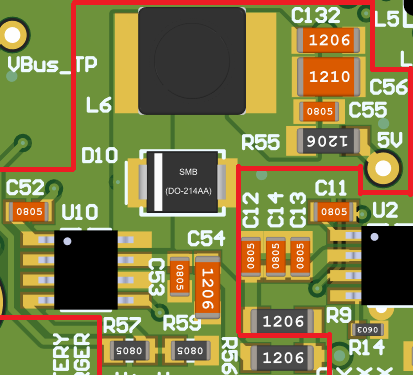
\includegraphics[width=0.5\textwidth]{figures/payloads-buck-circuit-3d.png}
        \caption{Payloads regulator circuit on the PCB.}
        \label{fig:payloads-buck-circuit-3d}
    \end{center}
\end{figure}

\section{External Connectors}

The EPS2 module is connected to the other modules using the PC104 bus. The solar panels, the kill-switches, the remove before flight, the RTDs, the heater, the batteries charger connector and the JTAG pins are connected using Molex PicoBlade connectors. The EPS2 module also has a jumper that connects the MCU VCC to the JTAG VCC and a header to debug the board via UART protocol. In the following sections each connector is detailed, with a picture showing the location on the EPS2 PCB and a table explaining each pin function.

\subsection{PC104} \label{PC104}

The connector referred as PC-104 is a junction of two double row 28H headers (\textit{SSW-126-01-G-D}). These connectors create a solid 104-pin interconnection across the different satellite modules. The \autoref{fig:pc104-scheme} shows the PC-104 interface from the bottom side of the PCB, which allows visualize the simplified label scheme in the board. Also, the \autoref{tab:pc104-pins} provides the connector pinout\footnote{This pinout is simplified since additional interfaces were omitted. Refer to \textit{option sheet} in chapter \ref{ch:assembly}.} for the pins that are connected to the module. 

\begin{figure}[!ht]
    \begin{center}
        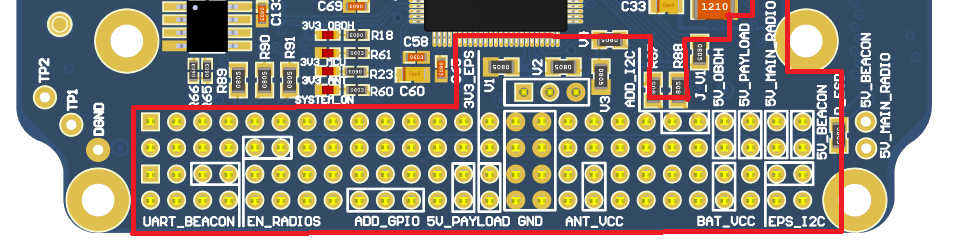
\includegraphics[width=0.8\textwidth]{figures/eps2_pc104_scheme.png}
        \caption{Bottom view of PC-104 and simplified labels.}
        \label{fig:pc104-scheme}
    \end{center}
\end{figure}

\begin{table}[!h]
    \centering
    \begin{tabular}{cllll}
        \toprule[1.5pt]
        \textit{Pin [A-B]} & \textit{H1A}     & \textit{H1B}     & \textit{H2A}  & \textit{H2B}  \\
        \midrule
        1-2                & -                & -                & -             & -             \\
        3-4                & -                & -                & -             & -             \\
        5-6                & -                & -                & UART\_RX      & -             \\
        7-8                & -                & -                & UART\_TX      & -             \\
        9-10               & -                & EN\_PWR\_5       & -             & -             \\
        11-12              & -                & EN\_PWR\_6       & -             & -             \\
        13-14              & -                & -                & -             & -             \\
        15-16              & -                & -                & -             & -             \\
        17-18              & -                & -                & -             & -             \\
        19-20              & -                & -                & -             & -             \\
        21-22              & -                & -                & -             & -             \\
        23-24              & -                & -                & -             & -             \\
        25-26              & -                & -                & PWR\_4\_5V    & PWR\_4\_5V    \\
        27-28              & -                & -                & PWR\_7\_3V3   & PWR\_7\_3V3   \\
        29-30              & GND              & GND              & GND           & GND           \\
        31-32              & GND              & GND              & GND           & GND           \\
        33-34              & -                & -                & -             & -             \\
        35-36              & -                & -                & PWR\_1\_3V3   & PWR\_1\_3V3   \\
        37-38              & -                & -                & -             & -             \\
        39-40              & -                & -                & -             & -             \\
        41-42              & -                & -                & -             & -             \\
        43-44              & -                & -                & -             & -             \\
        45-46              & PWR\_2\_3V3      & PWR\_2\_3V3      & PWR\_3\_BAT   & PWR\_3\_BAT   \\
        47-48              & PWR\_4\_5V       & PWR\_4\_5V       & -             & -             \\
        49-50              & PWR\_5\_5V       & PWR\_5\_5V       & I2C\_SDA      & -             \\
        51-52              & PWR\_6\_6V       & PWR\_6\_6V       & I2C\_SCL      & -             \\
        \bottomrule[1.5pt]
    \end{tabular}
    \caption{PC-104 connector pinout.}
    \label{tab:pc104-pins}
\end{table}

\begin{table}[!h]
    \centering
    \begin{tabular}{lL{0.29\textwidth}L{0.47\textwidth}}
        \toprule[1.5pt]
        \textbf{Signal}  & \textbf{Pin(s)}            & \textbf{Description} \\
        \midrule
        GND              & H1-29, H1-30, H1-31, H1-32, H2-29, H2-30, H2-31, H2-32 & Ground reference \\
        PWR\_1\_3V3      & H2-35, H2-36               & Power bus 1, 3.3 V, 2 A max. \\
        PWR\_2\_3V3      & H1-45, H1-46               & Power bus 2, 3.3 V, 1 A max. \\
        PWR\_3\_BAT      & H2-45, H2-46               & Power bus 3, battery terminals (+) \\
        PWR\_4\_5V       & H1-47, H1-48, H2-25, H2-26 & Power bus 4, 5 V, 3 A max. \\
        PWR\_5\_5V       & H1-49, H1-50               & Power bus 5, 5 V, 5 A max. \\
        PWR\_6\_6V       & H1-51, H1-52               & Power bus 6, 6 V, 5 A max. \\
        PWR\_7\_3V3      & H2-27, H2-28               & Power bus 7, 3.3 V, 2 A max. \\
        I2C\_SDA         & H2-49                      & Primary communication bus (data signal) \\
        I2C\_SCL         & H2-51                      & Primary communication bus (clock signal) \\
        UART\_RX         & H2-5                       & Secondary communication bus (RX) \\
        UART\_TX         & H2-7                       & Secondary communication bus (TX) \\
        EN\_PWR\_5       & H1-10                      & Enable signal of the power bus 5 \\
        EN\_PWR\_6       & H1-12                      & Enable signal of the power bus 6 \\
        \bottomrule[1.5pt]
    \end{tabular}
    \caption{PC-104 bus signal description.}
    \label{tab:pc104-signals}
\end{table}

\subsection{Solar Panels PicoBlades} \label{solar-panels-picoblades}

There are six PicoBlade connectors that can be connected to solar panels. Each one of them is to be used with its respective positive or negative cartesian axis reference label: X, Y or Z. Note that the total current for each individual PicoBlade pin must not exceed 1000mA, this means that the maximum current per connector is 2000mA.
Their pinout is showed in \autoref{tab:solar-panels-picoblades} and position on the PCB in \autoref{fig:solar-panels-picoblades}.

\begin{table}[!h]
    \centering
    \begin{tabular}{cl}
        \toprule[1.5pt]
        \textit{Pin} & \textit{Row} \\
        \midrule
        1            & Panel [side reference] positive input\\
        2            & Panel [side reference] positive input \\
        3            & PGND \\
        4            & PGND \\
        \bottomrule[1.5pt]
    \end{tabular}
    \caption{Solar panels PicoBlades pinout.}
    \label{tab:solar-panels-picoblades}
\end{table}

\begin{figure}[!ht]
    \begin{center}
        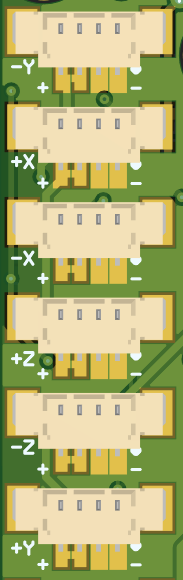
\includegraphics[width=0.2\textwidth]{figures/solar-panels-picoblades-3d.png}
        \caption{Solar panels power input connectors on the PCB.}
        \label{fig:solar-panels-picoblades}
    \end{center}
\end{figure}

\subsection{Kill-Switches PicoBlades} \label{kill-switches-picoblades}

There are two PicoBlade connectors to be connected to two separete kill-switch spring button mechanisms, one of the mechanism is ilustrated in \autoref{fig:kill-switch-installed}. The connection is done by manually soldering and isolating with a heat shrink tube, the other end of the cable goes to PicoBlades of the EPS, their pinout is showed in \autoref{tab:kill-switches-picoblades} and position on the PCB in \autoref{fig:kill-switches-picoblades}.

\begin{figure}[!ht]
    \begin{center}
        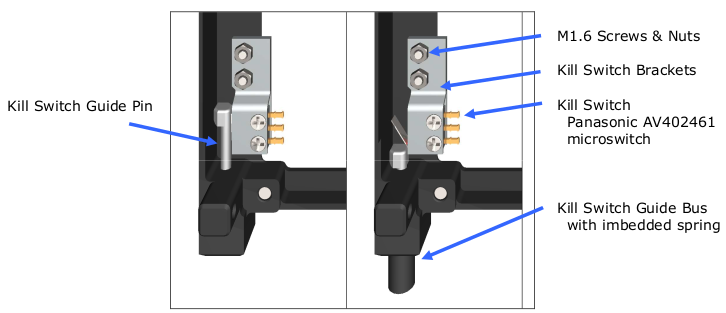
\includegraphics[width=\textwidth]{figures/kill-switch-installed.png}
        \caption{Kill-switch spring button mechanism.}
        \label{fig:kill-switch-installed}
    \end{center}
\end{figure}

\begin{table}[!h]
    \centering
    \begin{tabular}{cl}
        \toprule[1.5pt]
        \textit{Pin} & \textit{Row} \\
        \midrule
        1            & Common \\
        2            & Common \\
        3            & NO\nomenclature{\textbf{NO}}{\textit{Normally open.}} \\
        4            & NO\nomenclature{\textbf{NO}}{\textit{Normally open.}} \\
        5            & NC\nomenclature{\textbf{NC}}{\textit{Normally closed.}} \\
        6            & NC\nomenclature{\textbf{NC}}{\textit{Normally closed.}} \\
        \bottomrule[1.5pt]
    \end{tabular}
    \caption{Kill-switches PicoBlades pinout.}
    \label{tab:kill-switches-picoblades}
\end{table}

\begin{figure}[!ht]
    \begin{center}
        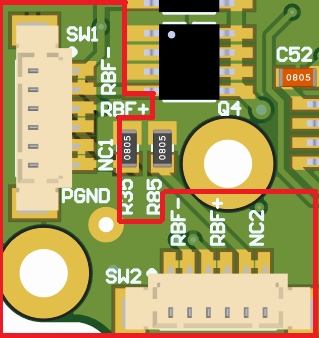
\includegraphics[width=0.35\textwidth]{figures/kill-switches-picoblades-3d.png}
        \caption{Kill-switches PicoBlade connectors on the PCB.}
        \label{fig:kill-switches-picoblades}
    \end{center}
\end{figure}

\subsection{RBF PicoBlade} \label{rbf-picoblade}

The RBF PicoBlade interconects the separation switches circuit present on the EPS to be acessed in a external interface. Its pinout is showed in \autoref{tab:rbf-picoblade} and position on the PCB in \autoref{fig:rbf-picoblade}.

\begin{table}[!h]
    \centering
    \begin{tabular}{cl}
        \toprule[1.5pt]
        \textit{Pin} & \textit{Row} \\
        \midrule
        1            & $+$RBF \\
        2            & $-$RBF \\
        3            & $+$RBF \\
        4            & $-$RBF \\
        \bottomrule[1.5pt]
    \end{tabular}
    \caption{RBF PicoBlade pinout.}
    \label{tab:rbf-picoblade}
\end{table}

\begin{figure}[!ht]
    \begin{center}
        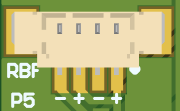
\includegraphics[width=0.25\textwidth]{figures/rbf-picoblades-3d.png}
        \caption{RBF PicoBlade connector on the PCB.}
        \label{fig:rbf-picoblade}
    \end{center}
\end{figure}

\subsection{RTDs PicoBlade} \label{rtd-picoblade}

EPS reads temperature from RTDs present in the BAT4C module with a external PicoBlade cable conected betweem both boards. The two connectors RTD1 and RTD2 pinouts are showed in \autoref{tab:rbf-picoblade} and positions on the PCB in \autoref{fig:rtds-picoblades}.

\begin{table}[!h]
    \centering
    \begin{tabular}{cl}
        \toprule[1.5pt]
        \textit{Pin} & \textit{Row} \\
        \midrule
        RTD1 PicoBlade &  \\
        \midrule
        1            & BAT\_GPIO1   \\
        2            & BAT\_GPIO2   \\
        3            & RTD\_Common  \\
        4            & RTD\_RTD3    \\
        5            & RTD\_Common  \\
        6            & RTD\_RTD2    \\
        7            & RTD\_Common  \\
        8            & RTD\_RTD6    \\
        \midrule
        RTD2 PicoBlade &  \\
        \midrule
        1            & RTD\_Common  \\
        2            & RTD\_RTD5    \\
        3            & RTD\_Common  \\
        4            & RTD\_RTD4    \\
        5            & RTD\_Common  \\
        6            & RTD\_RTD1    \\
        7            & RTD\_Common  \\
        8            & RTD\_RTD0    \\
        \bottomrule[1.5pt]
    \end{tabular}
    \caption{RBF PicoBlade pinout.}
    \label{tab:rbf-picoblade}
\end{table}

\begin{figure}[!ht]
    \begin{center}
        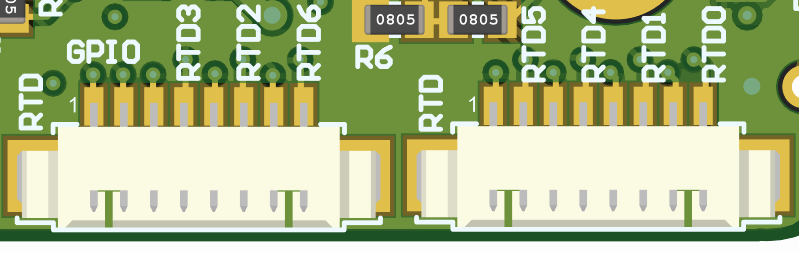
\includegraphics[width=0.45\textwidth]{figures/rtds-picoblades-3d.png}
        \caption{RTDs PicoBlade connectors on the PCB.}
        \label{fig:rtds-picoblades}
    \end{center}
\end{figure}

\subsection{Heater PicoBlade} \label{heater-picoblade}

The PWM signals that control the heaters present on the BAT4C module is also brought by a external PicoBlade cable. The connector pinout is showed in \autoref{tab:heater-picoblade} and positions on the PCB in \autoref{fig:heaters-picoblade}.

\begin{table}[!h]
    \centering
    \begin{tabular}{cl}
        \toprule[1.5pt]
        \textit{Pin} & \textit{Row} \\
        \midrule
        1            & $-$Heater1\_Voltage \\
        2            & $-$Heater1\_Voltage \\
        3            & VBUS \\
        4            & VBUS \\
        5            & $-$Heater2\_Voltage \\
        6            & $-$Heater2\_Voltage \\
        7            & VBUS \\
        8            & VBUS \\
        \bottomrule[1.5pt]
    \end{tabular}
    \caption{Heater PicoBlade pinout.}
    \label{tab:heater-picoblade}
\end{table}

\begin{figure}[!ht]
    \begin{center}
        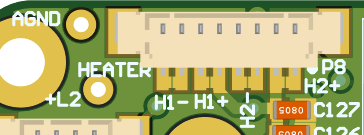
\includegraphics[width=0.4\textwidth]{figures/heaters-picoblade-3d.png}
        \caption{Heaters PicoBlade connector on the PCB.}
        \label{fig:heaters-picoblade}
    \end{center}
\end{figure}

\subsection{External Batteries Charger PicoBlade} \label{external-charge-picoblade}

When the EPS and BAT4C are assembled together the batteries can be charged from a PicoBlade connector on which is acessed in a external interface. The same current restriction as for the solar panels connectors is apllied here, the external batteries charger PicoBlade must not exceed 2000mA. The connector pinout is showed in \autoref{tab:batteries-picoblade} and position on the PCB in \autoref{fig:batteries-picoblade}.

\begin{table}[!h]
    \centering
    \begin{tabular}{cl}
        \toprule[1.5pt]
        \textit{Pin} & \textit{Row} \\
        \midrule
        1            & V\_Charging\_Batteries \\
        2            & V\_Charging\_Batteries \\
        3            & PGND \\
        4            & PGND \\
        \bottomrule[1.5pt]
    \end{tabular}
    \caption{External batteries charger PicoBlade pinout.}
    \label{tab:batteries-picoblade}
\end{table}

\begin{figure}[!ht]
    \begin{center}
        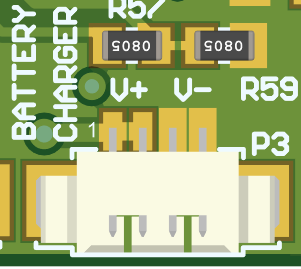
\includegraphics[width=0.25\textwidth]{figures/battery-charger-picoblade-3d.png}
        \caption{External batteries charger PicoBlade connector on the PCB.}
        \label{fig:batteries-picoblade}
    \end{center}
\end{figure}

\subsection{JTAG PicoBlade} \label{jtag-picoblade}

The EPS module can be programed and debugged through its JTAG PicoBlade connector, see \autoref{ch:instructions} for more information regarding right use of this interface. The connector pinout is showed in \autoref{tab:jtag-picoblade} and position on the PCB in \autoref{fig:jtag-picoblade}.

\begin{table}[!h]
    \centering
    \begin{tabular}{cl}
        \toprule[1.5pt]
        \textit{Pin} & \textit{Row} \\
        \midrule
        1            & 3V3\_MCU \\
        2            & TDO \\
        3            & TCK \\
        4            & UART\_Debug\_Tx \\
        5            & UART\_Debug\_Rx \\
        6            & DGND \\
        \bottomrule[1.5pt]
    \end{tabular}
    \caption{JTAG PicoBlade pinout.}
    \label{tab:jtag-picoblade}
\end{table}

\begin{figure}[!ht]
    \begin{center}
        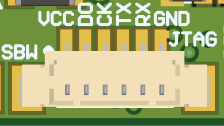
\includegraphics[width=0.35\textwidth]{figures/jtag-picoblade-3d.png}
        \caption{JTAG PicoBlade connector on the PCB.}
        \label{fig:jtag-picoblade}
    \end{center}
\end{figure}

\subsection{Debug UART Pin Header} \label{uart-pin-header}

For debugging via UART using log messages during test phase a pin header can be easily acessed with jumper wires. This connector is not meant to be soldered in the flight model of the EPS. The connector pinout is showed in \autoref{tab:uart-pin-header} and position on the PCB in \autoref{fig:uart-pin-header}.

\begin{table}[!h]
    \centering
    \begin{tabular}{cl}
        \toprule[1.5pt]
        \textit{Pin} & \textit{Row} \\
        \midrule
        1            & UART\_Debug\_Tx \\
        2            & UART\_Debug\_Rx \\
        3            &  DGND \\
        \bottomrule[1.5pt]
    \end{tabular}
    \caption{Debug UART pin header pinout.}
    \label{tab:uart-pin-header}
\end{table}

\begin{figure}[!ht]
    \begin{center}
        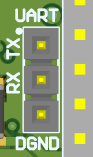
\includegraphics[width=0.15\textwidth]{figures/uart-pin-header-3d.png}
        \caption{Debug UART pin header connector on the PCB.}
        \label{fig:uart-pin-header}
    \end{center}
\end{figure}
    %
% firmware.tex
%
% Copyright (C) 2021 by SpaceLab.
%
% EPS 2.0 Documentation
%
% This work is licensed under the Creative Commons Attribution-ShareAlike 4.0
% International License. To view a copy of this license,
% visit http://creativecommons.org/licenses/by-sa/4.0/.
%

%
% \brief Firmware project chapter.
%
% \author Gabriel Mariano Marcelino <gabriel.mm8@gmail.com>
% \author Yan castro de Azeredo <yan.ufsceel@gmail.com>
%
% \institution Universidade Federal de Santa Catarina (UFSC)
%
% \version 0.1.0
%
% \date 2021/03/07
%

\chapter{Firmware} \label{ch:firmware}

\section{Dependencies}

\section{Tasks}

A list of the firmware tasks can be seen in the \autoref{tab:firmware-tasks}.

\begin{table}[!h]
    \centering
    \begin{tabular}{lccccc}
        \toprule[1.5pt]
        \textbf{Name}          & \textbf{Priority} & \textbf{Initial delay [ms]} & \textbf{Period [ms]} & \textbf{Stack [bytes]} \\
        \midrule
        Startup (boot)         & Highest           & 0                           & Aperiodic            & 500                    \\
        Watchdog reset         & Lowest            & 0                           & 100                  & 128                    \\
        Heartbeat              & Lowest            & 0                           & 500                  & 128                    \\
        System reset           & High              & 0                           & 36000000             & 128                    \\
        Battery Heater Control & TBD               & 0                           & TBD                  & TBD                    \\
        Read sensors           & Medium            & 0                           & 60000                & 128                    \\
        CSP Server             & Lowest            & 0                           & 500                  & 1024                   \\
        MPPT                   & TBD               & TBD                         & TBD                  & TBD                    \\
        Beacon package         & TBD               & TBD                         & TBD                  & TBD                    \\
        OBDH package           & Highest           & 4500   & Called by ISR\nomenclature{\textbf{ISR}}{\textit{Interrupt Service Routine.}}   & TBD \\
        \bottomrule[1.5pt]
    \end{tabular}
    \caption{Firmware tasks.}
    \label{tab:firmware-tasks}
\end{table}

\subsection{Startup (boot)}

\subsection{Watchdog reset}

\subsection{Heartbeat}

\subsection{System reset}

\subsection{Battery heater control}

\subsection{Read sensors}

\subsection{MPPT}

\subsection{Beacon package}

\subsection{OBDH package}

\section{Variables and Parameters}

A list of all the variables of EPS with their identification number (ID) and variable type that can be read from the sensors and peripherals is seen in the \autoref{tab:eps2-variables}.

\begin{longtable}[c]{cL{0.72\textwidth}lc}
    \toprule[1.5pt]
    \textbf{ID} & \textbf{Name/Description} & \textbf{Type} & \textbf{Access} \\
    \midrule
    0   & Time counter in millseconds                                       & uint32 & R \\
    1   & Temperature of the $\mu$C in K                                    & uint16 & R \\
    2   & EPS circuitry and Beacon MCU current in mA                        & uint16 & R \\
    \multirow{18}{*}{3} & Last reset cause: & \multirow{18}{*}{uint8} & \multirow{18}{*}{R} \\
        & - 0x00 = No interrupt pending                                     &        &  \\
        & - 0x02 = Brownout (BOR)                                           &        &  \\
        & - 0x04 = RST/NMI (BOR)                                            &        &  \\
        & - 0x06 = PMMSWBOR (BOR)                                           &        &  \\
        & - 0x08 = Wakeup from LPMx.5 (BOR)                                 &        &  \\
        & - 0x0A = Security violation (BOR)                                 &        &  \\
        & - 0x0C = SVSL (POR)                                               &        &  \\
        & - 0x0E = SVSH (POR)                                               &        &  \\
        & - 0x10 = SVML\_OVP (POR)                                          &        &  \\
        & - 0x12 = SVMH\_OVP (POR)                                          &        &  \\
        & - 0x14 = PMMSWPOR (POR)                                           &        &  \\
        & - 0x16 = WDT time out (PUC)                                       &        &  \\
        & - 0x18 = WDT password violation (PUC)                             &        &  \\
        & - 0x1A = Flash password violation (PUC)                           &        &  \\
        & - 0x1C = Reserved                                                 &        &  \\
        & - 0x1E = PERF peripheral/configuration area fetch (PUC)           &        &  \\
        & - 0x20 = PMM password violation (PUC)                             &        &  \\
        & - 0x22 to 0x3E = Reserved                                         &        &  \\
    4   & Reset counter                                                     & uint16 & R \\
    5   & -Y and +X sides solar panel voltage in mV                         & uint16 & R \\
    6   & -X and +Z sides solar panel voltage in mV                         & uint16 & R \\
    7   & -Z and +Y sides solar panel voltage in mV                         & uint16 & R \\
    8   & -Y side solar panel current in mA                                 & uint16 & R \\
    9   & +Y side solar panel current in mA                                 & uint16 & R \\
    10  & -X side solar panel current in mA                                 & uint16 & R \\
    11  & +X side solar panel current in mA                                 & uint16 & R \\
    12  & -Z side solar panel current in mA                                 & uint16 & R \\
    13  & +Z side solar panel current in mA                                 & uint16 & R \\
    14  & MPPT 1 duty cycle in \% (writable just in manual mode)            & uint8  & R/W \\
    15  & MPPT 2 duty cycle in \% (writable just in manual mode)            & uint8  & R/W \\
    16  & MPPT 3 duty cycle in \% (writable just in manual mode)            & uint8  & R/W \\
    17  & Total solar panels output voltage after MPPT in mV                & uint16 & R \\
    18  & Main power bus voltage in mV                                      & uint16 & R \\
    19  & RTD0 temperature in K                                             & uint32 & R \\
    20  & RTD1 temperature in K                                             & uint32 & R \\
    21  & RTD2 temperature in K                                             & uint32 & R \\
    22  & RTD3 temperature in K                                             & uint32 & R \\
    23  & RTD4 temperature in K                                             & uint32 & R \\
    24  & RTD5 temperature in K                                             & uint32 & R \\
    25  & RTD6 temperature in K                                             & uint32 & R \\
    26  & Batteries voltage in mV                                           & uint16 & R \\
    27  & Batteries current in mA                                           & uint16 & R \\
    28  & Batteries average current in mA                                   & uint16 & R \\
    29  & Batteries accumulated current in mA                               & uint16 & R \\
    30  & Batteries charge in mAh                                           & uint16 & R \\
    31  & Battery monitor IC temperature in K                               & uint16 & R \\
    32  & Battery monitor status register                                   & uint8  & R \\
    33  & Battery monitor protection register                               & uint8  & R \\
    34  & Battery monitor cycle counter                                     & uint8  & R \\
    35  & Battery monitor Remaining Active-Absolute Capacity (RAAC) in mAh  & uint16 & R \\
    36  & Battery monitor Remaining Standby-Absolute Capacity (RSAC) in mAh & uint16 & R \\
    37  & Battery monitor Remaining Active-Relative Capacity (RARC) in \%   & uint8  & R \\
    38  & Battery monitor Remaining Standby-Relative Capacity (RSRC) in \%  & uint8  & R \\
    39  & Battery heater 1 duty cycle in \% (writable just in manual mode)  & uint8  & R/W \\
    40  & Battery heater 2 duty cycle in \% (writable just in manual mode)  & uint8  & R/W \\
    41  & Hardware version                                                  & uint8  & R \\
    42  & Firmware version (ex.: ``v1.2.3''' = 0x00010203)                  & uint32 & R \\
    43  & MPPT 1 mode (0x00 = automatic, 0x01 = manual)                     & uint8  & R/W \\
    44  & MPPT 2 mode (0x00 = automatic, 0x01 = manual)                     & uint8  & R/W \\
    45  & MPPT 3 mode (0x00 = automatic, 0x01 = manual)                     & uint8  & R/W \\
    46  & Battery heater 1 mode (0x00 = automatic, 0x01 = manual)           & uint8  & R/W \\
    47  & Battery heater 2 mode (0x00 = automatic, 0x01 = manual)           & uint8  & R/W \\
    \bottomrule[1.5pt]
    \caption{Variables and parameters of the EPS 2.0.}
    \label{tab:eps2-variables}
\end{longtable}

\section{Operating System}

As operating system the FreeRTOS 10 \cite{freertos} is being used. FreeRTOS is a market-leading real-time operating system (RTOS) for microcontrollers and small microprocessors. Distributed freely under the MIT open source license, FreeRTOS includes a kernel and a growing set of IoT libraries suitable for use across all industry sectors. FreeRTOS is built with an emphasis on reliability and ease of use.

The main configuration parameters of the operating system in this project are availabe in \autoref{tab:freertos-config}.

\begin{table}[!h]
    \centering
    \begin{tabular}{lrr}
        \toprule[1.5pt]
        \textbf{Parameter}       & \textbf{Value} & \textbf{Unit} \\
        \midrule
        Version                  & v10.2.0        & - \\
        Tick rate (Hz)           & 1000           & Hz \\
        CPU clock (HZ)           & 32             & MHz \\
        Max. priorities          & TBD            & - \\
        Heap size                & TBD            & bytes \\
        Max. length of task name & 20             & - \\
        \bottomrule[1.5pt]
    \end{tabular}
    \caption{FreeRTOS main configuration parameters.}
    \label{tab:freertos-config}
\end{table}

More details of the used configuration parameters can be seen in the file \textit{\href{https://github.com/spacelab-ufsc/eps2/blob/master/firmware/config/FreeRTOSConfig.h}{firmware/config/FreeRTOSConfig.h}} from \cite{eps2}.

\section{Hardware Abstraction Layer (HAL)}

As the Hardware Abstraction Layer (HAL\nomenclature{\textbf{HAL}}{\textit{Hardware Abstraction Layer.}}), the DriverLib \cite{driverlib} from Texas Instruments is begin used. It is the official API to access the registers of the MSP430 microcontrollers.

The DriverLib is meant to provide a ``software'' layer to the programmer in order to facilitate higher level of programming compared to direct register accesses. By using the high level software APIs provided by DriverLib, users can create powerful and intuitive code which is highly portable between not only devices within the MSP430 platform, but between different families in the MSP430/MSP432 platforms.

    %
% assembly.tex
%
% Copyright (C) 2020 by SpaceLab.
%
% EPS 2.0 Documentation
%
% This work is licensed under the Creative Commons Attribution-ShareAlike 4.0
% International License. To view a copy of this license,
% visit http://creativecommons.org/licenses/by-sa/4.0/.
%

%
% \brief Assembly instructions chapter.
%
% \author Gabriel Mariano Marcelino <gabriel.mm8@gmail.com>
%
% \institution Universidade Federal de Santa Catarina (UFSC)
%
% \version 0.1.0
%
% \date 2020/11/05
%

\chapter{Board Assembly} \label{ch:assembly}

.

    %
% instructions.tex
%
% Copyright (C) 2021 by SpaceLab.
%
% EPS 2.0 Documentation
%
% This work is licensed under the Creative Commons Attribution-ShareAlike 4.0
% International License. To view a copy of this license,
% visit http://creativecommons.org/licenses/by-sa/4.0/.
%

%
% \brief Instructions chapter.
%
% \author Gabriel Mariano Marcelino <gabriel.mm8@gmail.com>
%
% \institution Universidade Federal de Santa Catarina (UFSC)
%
% \version 0.2.0
%
% \date 2020/11/05
%

\chapter{Usage Instructions} \label{ch:instructions}

\section{Powering the Board}

The EPS 2.0 is the energy provider module within a satellite, its nominal operation is alongside a battery pack from the BAT4C module and solar panels. 

During development and testing the board can also be partially powered using the JTAG interface (only the MCU and peripherals connected to the 3V3 EPS regulator), or fully powered directly through the battery connector with an equivalent power supply.

The module's PC104 power pins are available to be accessed externally, but it is advised to be used only for test probes and not powering directly from them. 

In the following subsections powering from the JTAG interface and batteries connector are explained in detail. 
It is advised to to have either the kill-switches on "NO" position and/or the RBF switch active before connecting the probes or cables to power the module.

% add real image of the IIP been used with EPS2
 
\subsection{Powering through JTAG Interface}

The JTAG interface is used for programming and debugging the module using a Flash Emulation Tool (refer to \autoref{jtag-picoblade} on the hardware chapter). 
This is done using a MSP-FET with the Spy-Bi-Wire protocol.
The tool should provide $3.3 V$ and a maximum of $100\ mA$, due to this current limitation only the EPS MCU can be powered for minimal testing and debugging purposes, for this the CN1 header pins must be shorted.
Remember that the CN1 connector should only be used if the EPS board is not being powered by any other means like batteries or external power supply.

For the interfacing the 14 pin cable of the MSP-FET to the EPS it is required an adapted cable or an external interface. 
The IIP\cite{iip} Nº1 and Nº2 boards have a 14 pin header that translates in a picoblade connector for the required connector counterpart on the EPS module, any of the pin header slots from 1 to 4 can be used.
When the MSP-FET is correctly connected and the necessary cable connections are done the kill-switches can be put on "NC" position and/or the RBF switch can be released.
The 3V3 MCU (refer to \autoref{status-leds} on the system overview chapter) indicates that the 3.3V power is being sourced, the system on led can be checked to see any easily dectable missbehavior right after the programming of the board. 
%On \autoref{eps-iip-connection} is showed the connection betweem EPS and IIP.


% add real image of the IIP been used with EPS2

\subsection{Powering through Power Supply}

To power the EPS module through external power supply, two voltage sources are needed.
The external power sources can be set up in two ways, either two \(3.7 V\) sources in series, or a \(3.7 V\) source for reference and a \(7.4 V\) source for power.
In both cases the voltage sources should be connected to one of the battery board connectors (P1 or P5).

To use two \(3.7 V\) sources, the first source should have it's negative and positive terminals connected to Vbat- and Vbat\_common pins of the batteries connector respectively, the second source should have it's negative and positive terminals connected to Vbat\_common and Vbat+ pins of the batteries connector respectively (refer to \autoref{fig:battery-connector} and \autoref{tab:battery-connector} on the hardware chapter).

To use \(3.7 V\) and \(7.4 V\) sources, the \(3.7 V\) source should have it's negative and positive terminals connected to Vbat- and Vbat\_common pins of the batteries connector respectively, the \(7.4 V\) source should have it's negative and positive terminals connected to Vbat- and Vbat+ pins of the batteries connector respectively (refer to \autoref{fig:battery-connector} and \autoref{tab:battery-connector} on the hardware chapter).

If the external power supply has configurable current limitation capability, it should be adjusted accordingly to the expected consumption of the load connected to the EPS module (other modules being powered by the EPS, batteries heaters being active, etc.), if powering the EPS in isolation (no load connected) a limit of \(80 mA\) may be applied.

After correctly connecting the voltage sources, the kill-switches can be put on "NC" position and/or the RBF switch can be released.

% add appendix instructions for equivalent power supply powering

\subsection{Powering through Batteries}

To power the EPS module from the batteries the BAT4C module must be connected through the P5 connector (refer to \autoref{fig:battery-connector} on the hardware chapter).
The batteries can be charged if needed using the P3 PicoBlade connector (refer to \autoref{external-charge-picoblade} on the hardware chapter), it will also required an external interface or an adapted cable to be used for interfacing the charger device to the PicoBlade.
The batteries also can be charged directly from the BAT4C module, for this refer to its documentation on the usage instruction chapter for more details \cite{bat4c}.


\section{Log Messages}

The EPS 2.0 has a UART interface dedicated for debugging, which is described in \autoref{tab:usci-config}. It follows a log system structure to improve the information provided in each message.
The messages can be acquired by connecting an USB cable to the IIP Nº3 board that has an integrated FTDI FT4232H IC \cite{iip}.

    %
% tests.tex
%
% Copyright (C) 2021 by SpaceLab.
%
% EPS 2.0 Documentation
%
% This work is licensed under the Creative Commons Attribution-ShareAlike 4.0
% International License. To view a copy of this license,
% visit http://creativecommons.org/licenses/by-sa/4.0/.
%

%
% \brief Test procedures chapter.
%
% \author Yan Castro de Azeredo <yan.ufsceel@gmail.com>
%
% \institution Universidade Federal de Santa Catarina (UFSC)
%
% \version 0.1.0
%
% \date 2021/04/24
%

\chapter{Test Procedures} \label{ch:test-procedures}

This chapter follows a standard worflow created by SpaceLab for testing its CubeSat modules, these procedures are first referenced in FloripaSat-2 documentation chapter 7\cite{floripasat2-doc}.
The \autoref{tab:test-procedures-table} resumes the workflow and each one of the tests types, substests and code identification. 
Some subtests can be considered to not be aplicable for the platform, the order in which they are done doesn't need to follow the numeration and other have generic titles that don't require too much explanation to be accomplished.     
The particularities of the EPS2 module for each test type are described in the following sections.

\begin{table}[!h]
    \centering
    \begin{tabular}{l|p{105mm}|p{5mm}}
        \toprule[1.5pt]
        Test type     & Subtests & ID \\
        \midrule
        A. Visual Inspection     & 1. Packaging quality assessment \newline 2. Board manufacturing and assembly quality \newline 3. 3D model comparison \newline 4. Layers marker \newline 5. Labels (schematics comparison) \newline 6. High resolution photos for documentation & TA1 \newline TA2 \newline TA3 \newline TA4 \newline TA5 \newline TA6 \\
        \midrule
        B. Mechanical Inspection     & 1. Board dimensions and mounting holes positioning \newline 2. Board weight measurement & TB1 \newline TB2 \\
        \midrule
        C. Integration Inspection    & 1. Check connectors pinout against the documentation \newline 2. Check connectors positioning & TC1 \newline TC2 \\
        \midrule
        D. Electrical Inspection     & 1. Solder shorts \newline 2. Missing components \newline 3. Lifted pins \newline 4. Poor soldering \newline 5. Swapped components \newline 6. Components partnumber & TD1 \newline TD2 \newline TD3 \newline TD4 \newline TD5 \newline TD6 \\
        \midrule
        E. Electrical Testing       & 1. Continuity test \newline 2. Power up procedures \newline 3. Average input power consumption measurement \newline 4. Average output power source measurement \newline 5. Power tracks temperature \newline 6. Simple signal integrity & TE1 \newline TE2 \newline TE3 \newline TE4 \newline TE5 \newline TE6 \\
        \midrule
        F. Functional Testing     & 1. Simple test code run \newline 2. System code run \newline 3. System hardware self-test flags check \newline 4. Monitor LEDs behavior \newline 5. Monitor the debug serial port logs & TF1 \newline TF2 \newline TF3 \newline TF4 \newline TF5 \\
         \midrule
        G. Visual Inspection     & 1. Review operation behavior \newline 2. Review features and requirements fulfillment \newline 3. Review communication buses configuration and protocol \newline 4. Review data packages, power buses and control signals \newline 5. Review edge cases and evaluate damage \newline 6. Run remote automated code tests \newline 7. Run system test codes in the board \newline 8. Run latest stable code version and review behavior & TG1 \newline TG2 \newline TG3 \newline TG4 \newline TG5 \newline TG6 \newline TG7 \newline TG8  \\
        \bottomrule[1.5pt]
    \end{tabular}
    \caption{Test workflow table.}
    \label{tab:test-procedures-table}
\end{table}

\section{Visual Inspection}

The first steps when receiving a manufactured (and in some cases assembled) PCB is to inspect visually to see if its according to its expected appereance. 
The EPS2 has more than 300 electrical components, so it is advised for this test to not take a long time to accomplish, the major noted problens should be spoted and reported. 
The \autoref{tab:visual-inspection} resumes the visual inspection steps. 

\begin{table}[!htb]
\centering
\caption{Visual Inspection test steps.}
\label{tab:visual-inspection}
\begin{tabular}{m{3cm} m{12cm} m{3cm}}
\toprule
Test type & Visual Inspection \\
\midrule
\midrule
Substests code & Description \\ 
\midrule
TA1 & Verify the received package, review the packaging protection used and if it maintained the physical and/or aesthetically integrity of the board. \\
\midrule
TA2 & See if the overall quality specified on the manufacturing process is according with its IPC class, the engineering model should be Class 2 while the flight model Class 3. \\
\midrule
TA3 & Inspect the top and bottom side of the PCB and verify if all the components are well soldered, if their polarity and labels are correct according to schematics and 3D model. Figure \ref{fig:pcb-top} and \ref{fig:pcb-bottom} for reference. If the board is not yet assembled detail the inconsistencies found during the assembly process. \\
\midrule
TA4 & Take a high resolution centred photo of the both sides of the board for documentation, avoid reflections if possible. \\
\midrule
\midrule
Success Criteria & The board needs to appear functional regarding its visual electrical specs. \\
\bottomrule
\end{tabular}
\end{table}

\section {Mechanical Inspection}

These tests verify if the board has the nominal mechanical specs prior to integration. 
The \autoref{tab:mechanical-inspection} resumes the mechanical inspection steps. 

\begin{table}[!htb]
\centering
\caption{Mechanical Inspection test steps.}
\label{tab:mechanical-inspection}
\begin{tabular}{m{3cm} m{12cm} m{3cm}}
\toprule
Test type & Mechanical Inspection \\
\midrule
\midrule
Substests code & Description \\ 
\midrule
TB1 & Verify board dimensions outline and mounting holes size and positioning with a measurement tool or through the board's draftsman sheet 1:1 scale print. \\
\midrule
TB2 & Measure board weight with an electronic balance with at least 0.1 grams of precision. \\
\midrule
\midrule
Success Criteria & The fabricated board needs to follow the mechanical specification of the draftsman document. \\
\bottomrule
\end{tabular}
\end{table}

\section{Integration Inspection}

These tests verify the integration accordance prior to the module's full assembly on the CubeSat.
The \autoref{tab:integration-inspection} resumes the integration inspection steps. 

\begin{table}[!htb]
\centering
\caption{Integration Inspection test steps.}
\label{tab:integration-inspection}
\begin{tabular}{m{3cm} m{12cm} m{3cm}}
\toprule
Test type & Integration Inspection \\
\midrule
\midrule
Substests code & Description \\ 
\midrule
TC1 & Check external connectors pinout labels againts the documentation present on \autoref{external-connectors}. \\
\midrule
TC2 & Check connectors positioning and possible integration issues from connected cables with the mounted BAT4C board and solar panels. \\
\midrule
\midrule
Success Criteria & The labels and placement of the external connectors must be according to the documentation and don't present any possible integration issues. \\
\bottomrule
\end{tabular}
\end{table}

\section {Electrical Inspection}

\section {Electrical Testing}

\section {Functional Testing}
 
\section {Module Testing}

    %
% references.tex
%
% Copyright (C) 2021 by SpaceLab.
%
% EPS 2.0 Documentation
%
% This work is licensed under the Creative Commons Attribution-ShareAlike 4.0
% International License. To view a copy of this license,
% visit http://creativecommons.org/licenses/by-sa/4.0/.
%

%
% \brief References chapter.
%
% \author Gabriel Mariano Marcelino <gabriel.mm8@gmail.com>
% \author Yan Castro de Azeredo <yan.ufsceel@gmail.com>
%
% \institution Universidade Federal de Santa Catarina (UFSC)
%
% \version 0.1.2
%
% \date 2021/03/16
%

\bibliography{references/floripasat2-doc,
			references/bat4c,
			references/eps-fsat,
			references/eps2,
			references/obdh2,
			references/msp430f6659,
			references/iip}

\addcontentsline{toc}{chapter}{References}

    %
% appendices.tex
%
% Copyright (C) 2021 by SpaceLab.
%
% EPS 2.0 Documentation
%
% This work is licensed under the Creative Commons Attribution-ShareAlike 4.0
% International License. To view a copy of this license,
% visit http://creativecommons.org/licenses/by-sa/4.0/.
%

%
% \brief Appendices.
%
% \author André M. P. Mattos <andre.mattos@spacelab.ufsc.com>
%
% \institution Universidade Federal de Santa Catarina (UFSC)
%
% \version 0.1.0
%
% \date 2021/06/23
%

\begin{appendices}

%
% test_report_v05.tex
%
% Copyright (C) 2021 by SpaceLab.
%
% EPS 2.0 Documentation
%
% This work is licensed under the Creative Commons Attribution-ShareAlike 4.0
% International License. To view a copy of this license,
% visit http://creativecommons.org/licenses/by-sa/4.0/.
%

%
% \brief Test report of the v0.1 hardware.
%
% \author André M. P. Mattos <andre.mattos@spacelab.ufsc.com>
%
% \institution Universidade Federal de Santa Catarina (UFSC)
%
% \version 0.1.0
%
% \date 2021/06/23
%

\chapter{Test Report of v0.1 Version} \label{anx:test-report-v01}

This appendix is a test report of the first manufactured and assembled PCB (version v0.1).

\begin{itemize}
    \item \textbf{PCB manufacturer}: PCBWay (China)
    \item \textbf{PCB assembly}: PCBWay (China)
    \item \textbf{PCB arrival date}: 2021/04/14
    \item \textbf{Execution date}: 2021/06/13 to 2021/07/01
    \item \textbf{Tester}: André M. P. Mattos
\end{itemize}



\section{Visual Inspection}

\begin{figure}[!ht]
    \begin{center}
        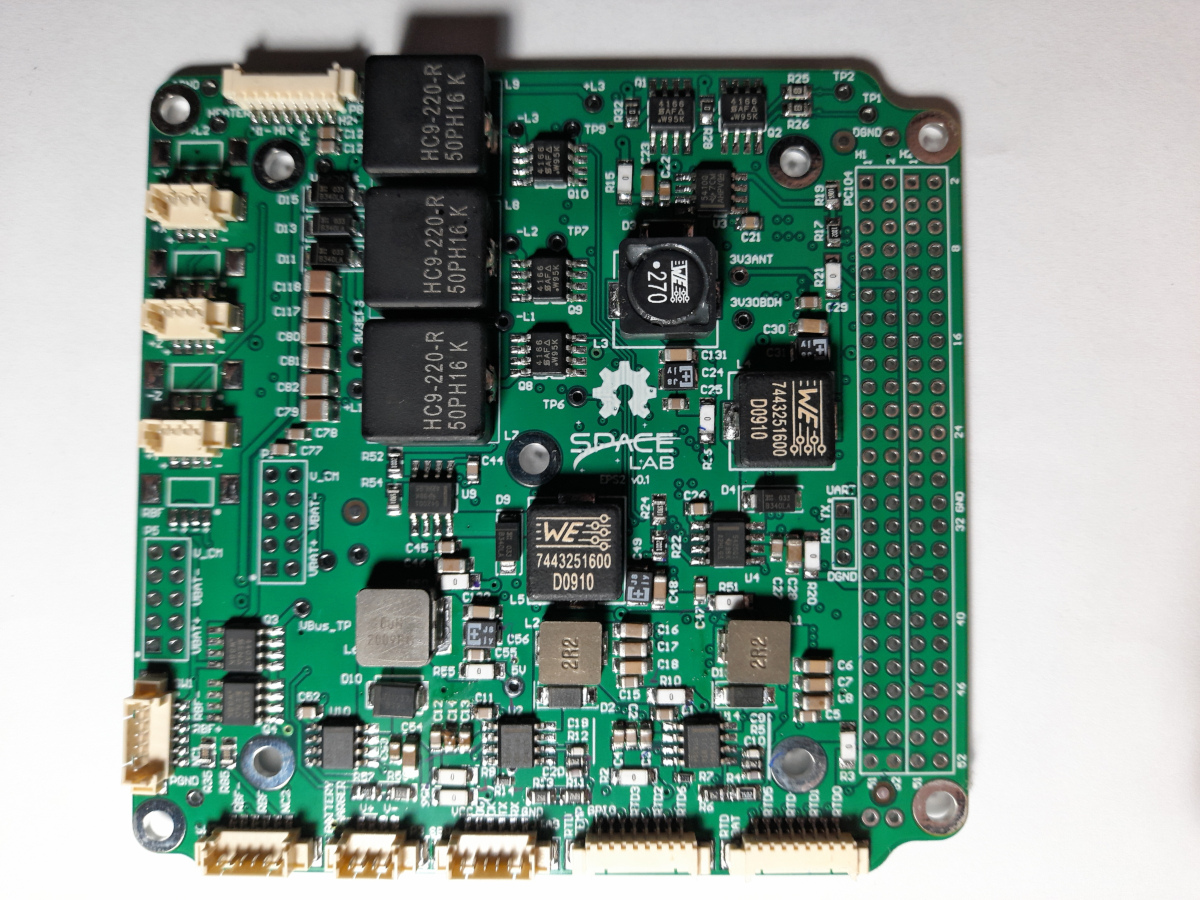
\includegraphics[width=0.75\columnwidth]{figures/v01/eps2-v01-top.jpg}
        \caption{Top view of the EPS 2.0 v0.1 board.}
        \label{fig:eps2-v01-top}
    \end{center}
\end{figure}

\begin{figure}[!ht]
    \begin{center}
        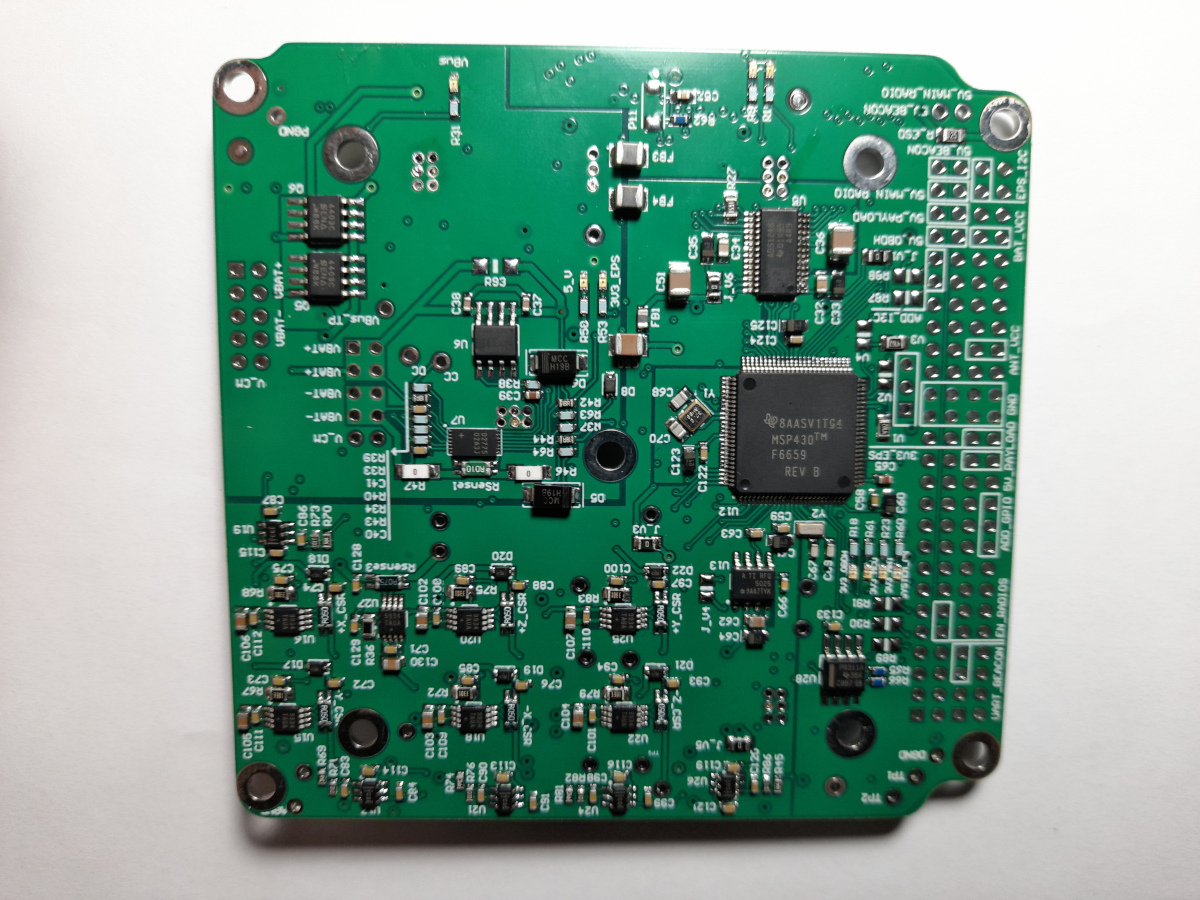
\includegraphics[width=0.75\columnwidth]{figures/v01/eps2-v01-bottom.jpg}
        \caption{Bottom view of the EPS 2.0 v0.1 board.}
        \label{fig:eps2-v01-bottom}
    \end{center}
\end{figure}

\begin{itemize}
    \item \textbf{Test description/Objective}: Inspection of the board, visually and with a multimeter, searching for fabrication and assembly failures.
    \item \textbf{Procedures:} \autoref{tab:visual-inspection}.
    \item \textbf{Material}: None.
    \item \textbf{Results}: The results of this test can be seen in Figures \ref{fig:eps2-v01-top} (top view of the board) and \ref{fig:eps2-v01-bottom} (bottom view of the board).
    \item \textbf{Conclusion}: No major problems were identified on this test, just some labels with typos (all in the PC-104 region) that should be already be corrected for v0.2 and four 4-pin picoblades that were not soldered by the manufacturer due the lack of clearance (differently from the headers and PC-104 which were intentionally removed from the process). This last item might be ignored since the manufacturer used an automated soldering process and the manual placement of these connectors is totally feasible.  
\end{itemize}

\section{Mechanical Inspection}

\begin{itemize}
    \item \textbf{Test description/Objective}: Evaluate if the board has the nominal mechanical specs prior to integration.
    \item \textbf{Procedures:} \autoref{tab:mechanical-inspection}.
    \item \textbf{Material}: None.
    \item \textbf{Results}: The inspection was not performed due to the lack of the proper tools.
    \item \textbf{Conclusion}: Even without the test, the board should not present any problem due to the heritage from the previous models and the good manufacturing quality.
\end{itemize}


\section{Integration Inspection}

\begin{itemize}
    \item \textbf{Test description/Objective}: Analyze the integration accordance prior to the module’s full assembly on the CubeSat.
    \item \textbf{Procedures:} \autoref{tab:integration-inspection}.
    \item \textbf{Material}: None.
    \item \textbf{Results}: Schematic files and pinouts identified in the \autoref{ch:hardware}. 
    \item \textbf{Conclusion}: No problems were identified on this test.
\end{itemize}


\section{Electrical Inspection}

\begin{itemize}
    \item \textbf{Test description/Objective}: Inspect the visually detectable electrical features.
    \item \textbf{Procedures:} \autoref{tab:electrical-inspection}.
    \item \textbf{Material}: None.
    \item \textbf{Results}: The results of this test can be seen in Figures \ref{fig:eps2-v01-top} (top view of the board) and \ref{fig:eps2-v01-bottom} (bottom view of the board).
    \item \textbf{Conclusion}: No problems were identified on this test, components were correctly selected, placed and soldered (except for those already mentioned in the visual inspection).
\end{itemize}


\section{Electrical Testing}

\begin{itemize}
    \item \textbf{Test description/Objective}: Perform basic tests to evaluate the board with nominal operating parameters.
    \item \textbf{Procedures:} \autoref{tab:electrical-testing}.
    \item \textbf{Material}:
        \begin{itemize}
            \item Multimeter Fluke 179
            \item Keysight N6705B DC Power Analyzer
        \end{itemize}
    \item \textbf{Results}: Results reported with the following images: \ref{fig:electrical-test-setup}, \ref{fig:power-consumption}, \ref{fig:regulator-payload}, \ref{fig:regulator-antenna}, \ref{fig:regulator-radio0}, \ref{fig:regulator-radio1}, \ref{fig:regulator-obdh} and \ref{fig:regulator-epsttc}. 
    \item \textbf{Conclusion}: The boards power-up as expected and present stable power consumption. The power outputs (step-down regulators) underperform with nominal or slightly higher load parameters. The issue might be related to poor sizing of passive components required for the regulators. This problem \textbf{must} be solved for the next version (it is expected to be performed minor changes in components values).  
\end{itemize}

\begin{figure}[!htb]
    \begin{center}
        \subfigure[Test setup for power characterization.\label{fig:electrical-test-tools}]{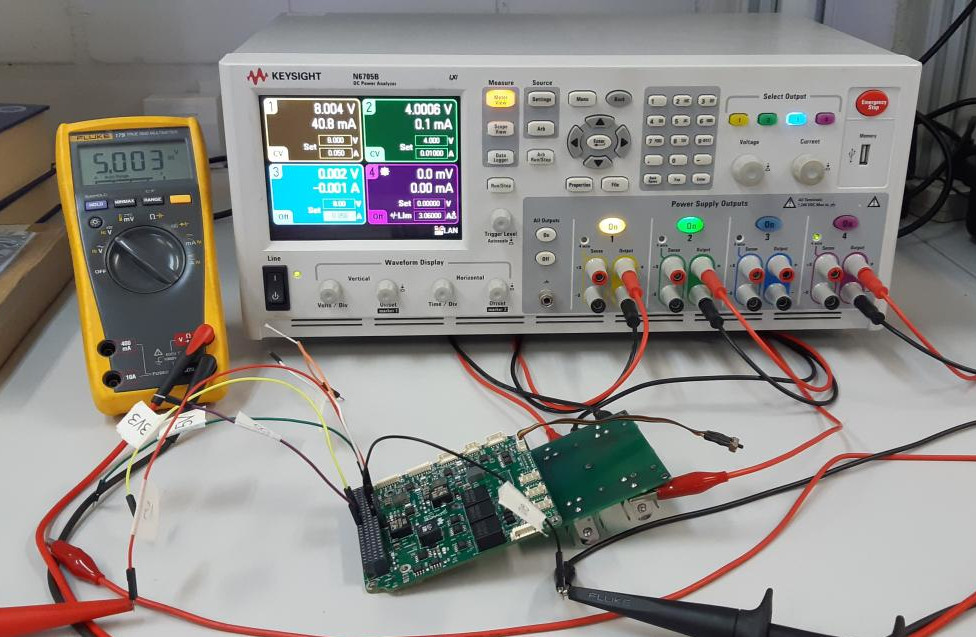
\includegraphics[height=0.28\textheight]{figures/v01/electrical-test-tools.jpg}}
        ~
        \subfigure[Board connectors and harness used during the tests.\label{fig:electrical-test-board}]{\includegraphics[height=0.28\textheight]{figures/v01/electrical-test-board.jpg}}
        \caption{Electrical test setup of the power-up sequence and output power supply channels.}
        \label{fig:electrical-test-setup}
    \end{center}
\end{figure}

\begin{figure}[!ht]
    \begin{center}
        \includegraphics[width=\columnwidth]{figures/v01/power-consumption.jpg}
        \caption{Power consumption during standby with any intensive firmware task.}
        \label{fig:power-consumption}
    \end{center}
\end{figure}

\begin{figure}[!htb]
    \begin{center}
        \subfigure[Load: 0mA.\label{fig:regulator-payload-0mA}]{\includegraphics[height=0.19\textheight]{figures/v01/regulator-payload-0mA.jpg}}
        ~
        \subfigure[Load: 500mA.\label{fig:regulator-payload-500mA}]{\includegraphics[height=0.19\textheight]{figures/v01/regulator-payload-500mA.jpg}}
        ~
        \subfigure[Load: 1000mA.\label{fig:regulator-payload-1000mA}]{\includegraphics[height=0.19\textheight]{figures/v01/regulator-payload-1000mA.jpg}}
        ~
        \subfigure[Load: 1500mA.\label{fig:regulator-payload-1500mA}]{\includegraphics[height=0.19\textheight]{figures/v01/regulator-payload-1500mA.jpg}}
        
        \caption{Payload step-down regulator power characterization.}
        \label{fig:regulator-payload}
    \end{center}
\end{figure}

\begin{figure}[!htb]
    \begin{center}
        \subfigure[Load: 0mA.\label{fig:regulator-antenna-0mA}]{\includegraphics[height=0.19\textheight]{figures/v01/regulator-antenna-0mA.jpg}}
        ~
        \subfigure[Load: 500mA.\label{fig:regulator-antenna-500mA}]{\includegraphics[height=0.19\textheight]{figures/v01/regulator-antenna-500mA.jpg}}
        ~
        \subfigure[Load: 1000mA.\label{fig:regulator-antenna-1000mA}]{\includegraphics[height=0.19\textheight]{figures/v01/regulator-antenna-1000mA.jpg}}
        ~
        \subfigure[Load: 1500mA.\label{fig:regulator-antenna-1500mA}]{\includegraphics[height=0.19\textheight]{figures/v01/regulator-antenna-1500mA.jpg}}
        
        \caption{Antenna step-down regulator power characterization.}
        \label{fig:regulator-antenna}
    \end{center}
\end{figure}

\begin{figure}[!htb]
    \begin{center}
        \subfigure[Load: 0mA.\label{fig:regulator-radio0-0mA}]{\includegraphics[height=0.19\textheight]{figures/v01/regulator-radio0-0mA.jpg}}
        ~
        \subfigure[Load: 500mA.\label{fig:regulator-radio0-500mA}]{\includegraphics[height=0.19\textheight]{figures/v01/regulator-radio0-500mA.jpg}}
        ~
        \subfigure[Load: 1000mA.\label{fig:regulator-radio0-1000mA}]{\includegraphics[height=0.19\textheight]{figures/v01/regulator-radio0-1000mA.jpg}}
        ~
        \subfigure[Load: 1500mA.\label{fig:regulator-radio0-1500mA}]{\includegraphics[height=0.19\textheight]{figures/v01/regulator-radio0-1500mA.jpg}}
        
        \caption{Radio 0 step-down regulator power characterization.}
        \label{fig:regulator-radio0}
    \end{center}
\end{figure}

\begin{figure}[!htb]
    \begin{center}
        \subfigure[Load: 0mA.\label{fig:regulator-radio1-0mA}]{\includegraphics[height=0.19\textheight]{figures/v01/regulator-radio1-0mA.jpg}}
        ~
        \subfigure[Load: 500mA.\label{fig:regulator-radio1-500mA}]{\includegraphics[height=0.19\textheight]{figures/v01/regulator-radio1-500mA.jpg}}
        ~
        \subfigure[Load: 1000mA.\label{fig:regulator-radio1-1000mA}]{\includegraphics[height=0.19\textheight]{figures/v01/regulator-radio1-1000mA.jpg}}
        ~
        \subfigure[Load: 1500mA.\label{fig:regulator-radio1-1500mA}]{\includegraphics[height=0.19\textheight]{figures/v01/regulator-radio1-1500mA.jpg}}
        
        \caption{Radio 1 step-down regulator power characterization.}
        \label{fig:regulator-radio1}
    \end{center}
\end{figure}

\begin{figure}[!htb]
    \begin{center}
        \subfigure[Load: 0mA.\label{fig:regulator-obdh-0mA}]{\includegraphics[height=0.19\textheight]{figures/v01/regulator-obdh-0mA.jpg}}
        ~
        \subfigure[Load: 500mA.\label{fig:regulator-obdh-100mA}]{\includegraphics[height=0.19\textheight]{figures/v01/regulator-obdh-100mA.jpg}}
        ~
        \subfigure[Load: 1000mA.\label{fig:regulator-obdh-200mA}]{\includegraphics[height=0.19\textheight]{figures/v01/regulator-obdh-200mA.jpg}}
        ~
        \subfigure[Load: 1500mA.\label{fig:regulator-obdh-500mA}]{\includegraphics[height=0.19\textheight]{figures/v01/regulator-obdh-500mA.jpg}}
        
        \caption{OBDH step-down regulator power characterization.}
        \label{fig:regulator-obdh}
    \end{center}
\end{figure}

\begin{figure}[!htb]
    \begin{center}
        \subfigure[Load: 0mA.\label{fig:regulator-epsttc-0mA}]{\includegraphics[height=0.19\textheight]{figures/v01/regulator-epsttc-0mA.jpg}}
        ~
        \subfigure[Load: 500mA.\label{fig:regulator-epsttc-500mA}]{\includegraphics[height=0.19\textheight]{figures/v01/regulator-epsttc-500mA.jpg}}
        ~
        \subfigure[Load: 1000mA.\label{fig:regulator-epsttc-1000mA}]{\includegraphics[height=0.19\textheight]{figures/v01/regulator-epsttc-1000mA.jpg}}

        \caption{EPS/TTC step-down regulator power characterization.}
        \label{fig:regulator-epsttc}
    \end{center}
\end{figure}
 
 \newpage

\section{Functional Testing}

\subsection{Firmware Programming}

\begin{itemize}
    \item \textbf{Test description/Objective}: Evaluate the board behavior under a firmware programming sequence.
    \item \textbf{Material}:
        \begin{itemize}
            \item Code Composer Studio v10.0.0
            \item MSP-FET Flash Emulation Tool
            \item USB-UART converter
            \item PuTTy
        \end{itemize}
    \item \textbf{Results}: The results of this are available in \autoref{fig:log-first-boot}, where the log messages of the first boot of the board can be seen.
    \item \textbf{Conclusion}: Major problems were identified on this test, but it was expected since the available firmware version was at early stages of refactoring and development.
\end{itemize}

\begin{figure}[!htb]
    \begin{center}
        \subfigure[Board connections using the MSP-FET and USB-UART converter.\label{fig:setup-first-boot}]{\includegraphics[height=0.2\textheight]{figures/v01/setup-first-boot.jpg}}
        ~
        \subfigure[Pin connections using the MSP-FET and USB-UART converter.\label{fig:electrical-test-board}]{\includegraphics[height=0.2\textheight]{figures/v01/tools-first-boot.jpg}}
        \caption{Setup used for the first firmware boot}
        \label{fig:setup-first-boot}
    \end{center}
\end{figure}

\begin{figure}[!ht]
    \begin{center}
        \includegraphics[width=0.4\columnwidth]{figures/v01/log-first-boot.png}
        \caption{Log messages during the first boot.}
        \label{fig:log-first-boot}
    \end{center}
\end{figure}

%\subsection{Communication Buses}
%
%\begin{itemize}
%    \item \textbf{Test description/Objective}: Test the communication busses of the board, as listed below:
%        \begin{itemize}
%            \item I$^{2}$C Port 0
%            \item I$^{2}$C Port 1
%            \item I$^{2}$C Port 2
%        \end{itemize}
%    \item \textbf{Material}:
%        \begin{itemize}
%            \item Saleae Logic Analyzer (24 MHz, 8 channels)
%            \item Saleae Logic software (v1.2.18)
%            \item MSP-FET Flash Emulation Tool
%        \end{itemize}
%    \item \textbf{Results}: The results of this test can be seen in Figures \ref{fig:test-i2c-0}, \ref{fig:test-i2c-1} and \ref{fig:test-i2c-2}.
%    \item \textbf{Conclusion:} No problems were identified on this test, all buses are working as expected.
%\end{itemize}
%
%\begin{figure}[!htb]
%    \begin{center}
%        \subfigure[Connections of the I$^{2}$C port 0 test.\label{fig:connections-i2c-0}]{\includegraphics[height=0.22\textheight]{figures/v05/test-i2c-0.jpg}}
%        ~
%        \subfigure[Waveforms of the I$^{2}$C port 0 test.\label{fig:waveform-i2c-0}]{\includegraphics[height=0.22\textheight]{figures/v05/waveform-i2c-0.png}}
%        \caption{I$^{2}$C port 0 test.}
%        \label{fig:test-i2c-0}
%    \end{center}
%\end{figure}
%
%
%
%\begin{figure}[!htb]
%    \begin{center}
%        \subfigure[Connections of the I$^{2}$C port 1 test.\label{fig:connections-i2c-1}]{\includegraphics[height=0.22\textheight]{figures/v05/test-i2c-1.jpg}}
%        ~
%        \subfigure[Waveforms of the I$^{2}$C port 1 test.\label{fig:waveform-i2c-1}]{\includegraphics[height=0.22\textheight]{figures/v05/waveform-i2c-1.png}}
%        \caption{I$^{2}$C port 1 test.}
%        \label{fig:test-i2c-1}
%    \end{center}
%\end{figure}
%
%
%
%\begin{figure}[!htb]
%    \begin{center}
%        \subfigure[Connections of the I$^{2}$C port 2 test.\label{fig:connections-i2c-2}]{\includegraphics[height=0.22\textheight]{figures/v05/test-i2c-2.jpg}}
%        ~
%        \subfigure[Waveforms of the I$^{2}$C port 2 test.\label{fig:waveform-i2c-2}]{\includegraphics[height=0.22\textheight]{figures/v05/waveform-i2c-2.png}}
%        \caption{I$^{2}$C port 2 test.}
%        \label{fig:test-i2c-2}
%    \end{center}
%\end{figure}
%
%\subsection{Sensors}
%
%\subsection{Input Voltage}
%
%\begin{itemize}
%    \item \textbf{Test description/Objective}: .
%    \item \textbf{Material}:
%        \begin{itemize}
%            \item Code Composer Studio v9.3.0
%            \item MSP-FET Flash Emulation Tool
%            \item USB-UART converter
%            \item Screen (Linux software)
%        \end{itemize}
%    \item \textbf{Results}: .
%    \item \textbf{Conclusion:} .
%\end{itemize}
%
%\subsection{Input Current}
%
%\begin{itemize}
%    \item \textbf{Test description/Objective}: .
%    \item \textbf{Material}:
%        \begin{itemize}
%            \item Code Composer Studio v9.3.0
%            \item MSP-FET Flash Emulation Tool
%            \item USB-UART converter
%            \item Screen (Linux software)
%        \end{itemize}
%    \item \textbf{Results}: .
%    \item \textbf{Conclusion:} .
%\end{itemize}
%
%\begin{figure}[!htb]
%    \begin{center}
%        \subfigure[Current sensing circuit.\label{fig:current-sensing-circuit-v05}]{\includegraphics[width=0.8\textwidth]{figures/v05/current-sensor-circuit.png}}
%
%        \subfigure[MAX9934 pinout.\label{fig:max9934-pinout}]{\includegraphics[width=0.4\textwidth]{figures/v05/max9934-top-view.png}}
%        ~
%        \subfigure[Current sensing layout (bottom layer).\label{fig:}]{\includegraphics[width=0.4\textwidth]{figures/v05/current-sensor-layout.png}}
%        \caption{.}
%        \label{fig:current-sensing-error-v05}
%    \end{center}
%\end{figure}
%
%\begin{figure}[!ht]
%    \begin{center}
%        \includegraphics[width=0.6\columnwidth]{figures/v05/max9934-fix.jpg}
%        \caption{Current sensor fix.}
%        \label{fig:current-sensor-fix}
%    \end{center}
%\end{figure}
%
%\begin{figure}[!ht]
%    \begin{center}
%        \includegraphics[width=0.7\columnwidth]{figures/v05/log-current-sensor.png}
%        \caption{Log messages with the read values from the current sensor.}
%        \label{fig:log-current-sensor}
%    \end{center}
%\end{figure}
%
%\subsection{Peripherals}
%
%\subsection{NOR Flash Memory}
%
%\begin{itemize}
%    \item \textbf{Test description/Objective}: Test the functionality of the NOR flash memory by verifying the device ID register of the IC.
%    \item \textbf{Material}:
%        \begin{itemize}
%            \item Saleae Logic Analyzer (24 MHz, 8 channels)
%            \item Saleae Logic software (v1.2.18)
%            \item MSP-FET Flash Emulation Tool
%        \end{itemize}
%    \item \textbf{Results}: The results of this test can be seen in \autoref{fig:test-nor-memory}.
%    \item \textbf{Conclusion:} No problems were identified on this test, as can be seen in \autoref{fig:waveform-spi-mem}, the device ID register was read as expected.
%\end{itemize}
%
%\begin{figure}[!htb]
%    \begin{center}
%        \subfigure[Connections of the NOR flash memory test.\label{fig:connections-nor-memory}]{\includegraphics[height=0.22\textheight]{figures/v05/test-nor-memory.jpg}}
%        ~
%        \subfigure[Waveforms of the NOR memory SPI.\label{fig:waveform-spi-mem}]{\includegraphics[height=0.22\textheight]{figures/v05/waveform-spi-mem.png}}
%        \caption{NOR memory SPI test.}
%        \label{fig:test-nor-memory}
%    \end{center}
%\end{figure}
%

\section{Conclusion}

The board needs to be tested more, to evaluate its functioning with the firmware that is being developed. 


\end{appendices}


\end{document}
